\graphicspath{{img/capture_leptons/}}
%%%%%%%%%%%%%%%%%%%%%%%%%%%%%%%%%%%%%
%%%%%%%%%%%%%%%%%%%%%%%%%%%%%%%%%%%%%
%%%%%%%%%%%%%%%%%%%%%%%%%%%%%%%%%%%%%

\chapter{Capture from Scattering on Leptonic Species in Compact Objects}
\label{chapter:capture_leptons}

\begin{synopsis}
This chapter is based on the results of Ref.~\cite{Bell:2020lmm_mar_ImprovedTreatmentDark} and on the electron capture results in Ref.~\cite{Bell:2021fye_oct_Improvedtreatmentdark}. We apply the formalism for capture in compact objects to leptonic targets in neutron stars and white dwarfs. In NSs, we calculate the projected sensitivities for the threshold DM-electron/muon cross-sections that could be probed in future observations. We then move to capture due to scattering with the electrons in WDs, where we analyse the existing observations of the WDs in the globular cluster M4. Limits are placed on the DM-electron cross-section by requiring that the DM does not heat up the WDs above their observed temperatures through scattering and annihilation.
\end{synopsis}
%%%%%%%%%%%%%%%%%%%%%%%%%%%%%%%%%%%%%
%%%%%%%%%%%%%%%%%%%%%%%%%%%%%%%%%%%%%
%%%%%%%%%%%%%%%%%%%%%%%%%%%%%%%%%%%%%



%%%%%%%%%%%%%%%%%%%%%%%%%%%%%%%%%%%%%
%%%%%%%%%%%%%%%%%%%%%%%%%%%%%%%%%%%%%

\section{Scattering on Leptons in Neutron Stars}
\label{ch4:sec:lep_NS}
%%%%%%%%%%%%%%%%%%%%%%%%%%%%%%%%%%%%%
%%%%%%%%%%%%%%%%%%%%%%%%%%%%%%%%%%%%%
Despite NSs being composed primarily of baryons (neutrons and protons in particular), they can still contain a substantial number of leptonic particles, namely electrons and, to a smaller extent, muons. The relative abundances of the species are determined by $\beta$-equlibrium as discussed in Section~\ref{ch2:sec:neutron_stars}. For example, 1.5 $\Msun$ NS can contain $\sim 5\times 10^{42}$ leptons, corresponding to a threshold cross-section $\sigmathl\sim 10^{-43}\cm^2$.

To that end, we will consider the BSk24 EoS, with the benchmark configurations listed in Table.~\ref{ch2:tab:BSk_configs}.
In Fig.~\ref{ch4:fig:NSradprofs1}, we plot the corresponding lepton profiles.
Electrons are present throughout the star, while muons begin to appear once the baryon number density exceeds $n_b\simeq 0.12\fm^{-3}$. The kink observed in the electron chemical potential marks out the transition from the core to the inner crust, where muons begin to appear. 

\begin{figure}[t] 
    \centering
    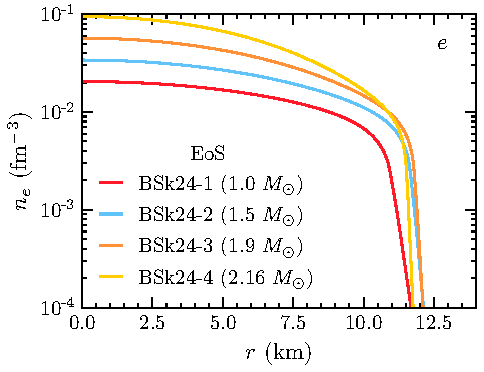
\includegraphics[width=0.495\textwidth]{capture_2/NS_ne_r_BSk24.pdf}
    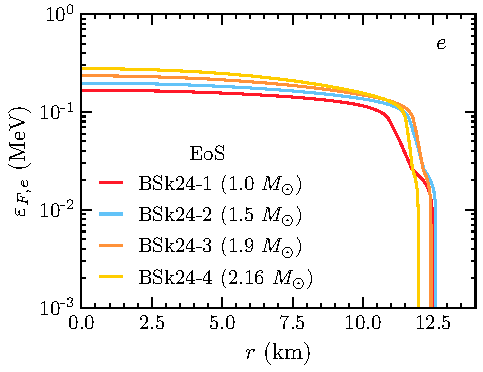
\includegraphics[width=0.495\textwidth]{capture_2/NS_MuFe_r_BSk24.pdf}
    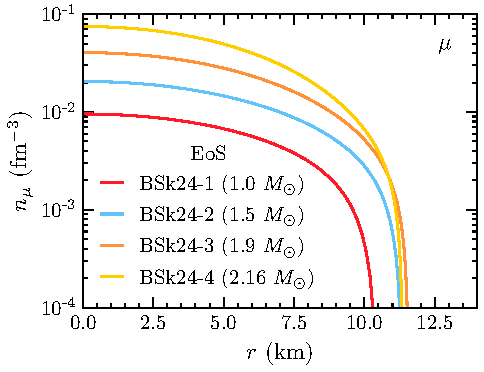
\includegraphics[width=0.495\textwidth]{capture_2/NS_nmu_r_BSk24.pdf}
    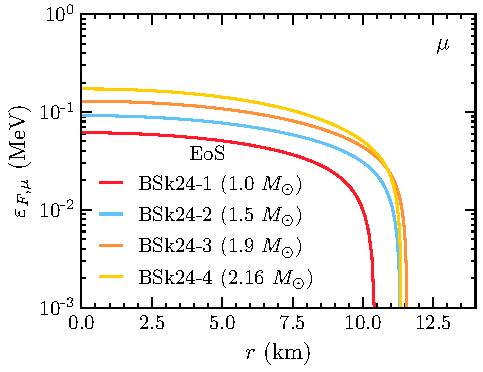
\includegraphics[width=0.495\textwidth]{capture_2/NS_MuFmu_r_BSk24.pdf}
    \caption{Number density profile (left) and chemical potential (right) for electrons (top) and muons (bottom) and NS configurations of the  BSk24 functional in Table~\ref{ch2:tab:BSk_configs}. 
    }
    \label{ch4:fig:NSradprofs1}
\end{figure}



%%%%%%%%%%%%%%%%%%%%%%%%%%%%%%%%%%%%%%%%%%%%%%%%%%%%%%%%%%%%%%%%%%%%%%%%%%%%%%%%%%%%
%%%%%%%%%%%%%%%%%%%%%%%%%%%%%%%%%%%%%%%%%%%%%%%%%%%%%%%%%%%%%%%%%%%%%%%%%%%%%%%%%%%%
\subsection{Capture Rate}
\label{ch4:subsec:caprateresults}
%%%%%%%%%%%%%%%%%%%%%%%%%%%%%%%%%%%%%%%%%%%%%%%%%%%%%%%%%%%%%%%%%%%%%%%%%%%%%%%%%%%%
%%%%%%%%%%%%%%%%%%%%%%%%%%%%%%%%%%%%%%%%%%%%%%%%%%%%%%%%%%%%%%%%%%%%%%%%%%%%%%%%%%%%

In this section, we present results for $C\Lambda^4$, the capture rate normalised by the EFT cutoff $\Lambda$, for each of the EFT operators in Table~\ref{ch1:tab:opers_defn_full}, calculated in the optically thin limit using Eq.~\ref{ch3:eq:capturefinalM2} for $m_\chi\lesssim m_\ell^*$ and  Eq.~\ref{ch3:eq:capturesimplelargem} for $m_\chi\gtrsim m_\ell^*$\footnote{To numerically solve these equations we use the \texttt{CUBA} libraries \cite{Hahn:2004fe_CUBALibrarymultidimensional, Hahn:2014fua_Concurrentcuba} linked to \texttt{Mathematica}~\cite{Mathematica}.}. Typical values of $m_\ell^\star$ and $\sigmathl$ are shown in Table.~\ref{ch4:tab:mstarsigma} for electron and muon targets. Note that $m_\ell^*$ will depend on the values of $B(r)$ and $\kinFl(r)$, as well as the type of interaction considered. 

\begin{figure}[t] 
    \centering
    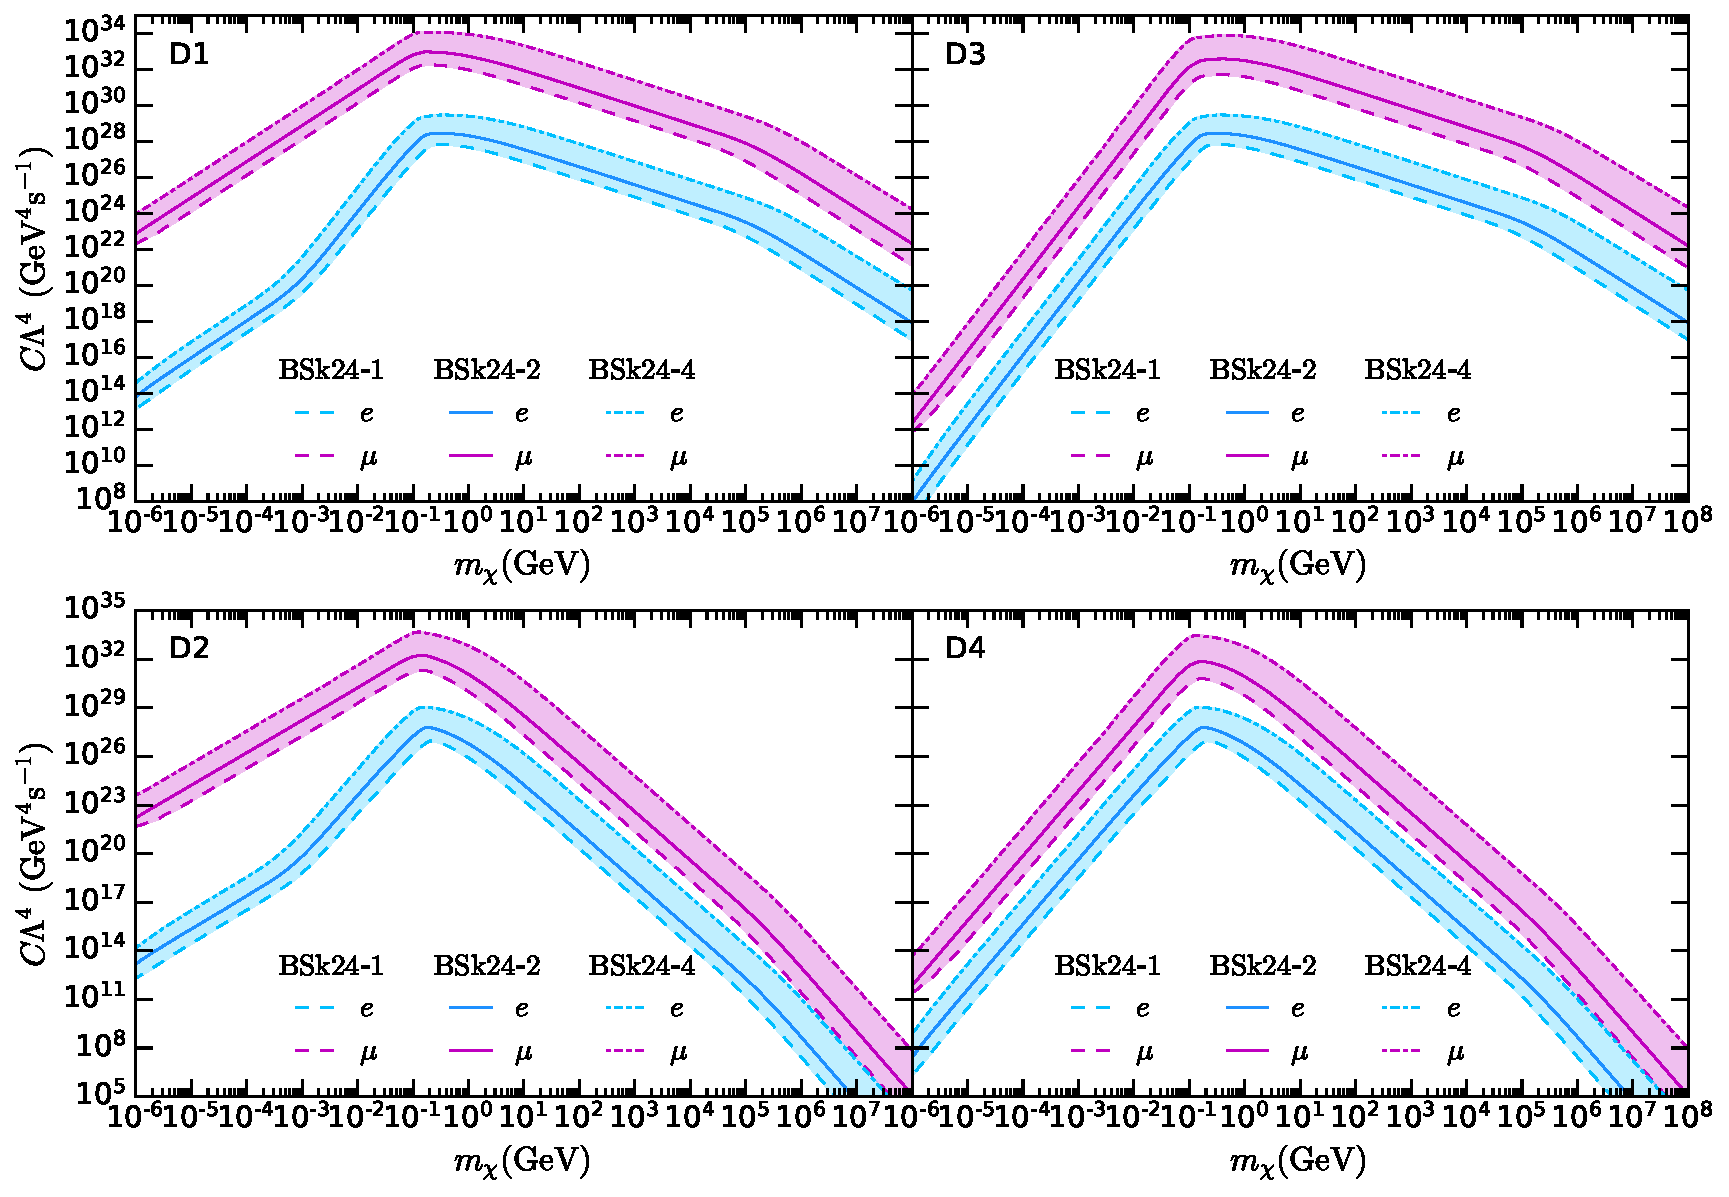
\includegraphics[width=\textwidth]{capture_2/D1_D4_C_mDM_lept.pdf}
    \caption[Capture rate in the optically thin limit for operators D1-D4 as a function of the DM mass $m_\chi$ for electrons (light blue) and muons (magenta) in the NS benchmark models BSk24-1 (dashed), BSk24-2 (solid) and BSk24-4 (dot-dashed).]{Capture rate in the optically thin limit for operators D1-D4 as a function of the DM mass $m_\chi$ for electrons (light blue) and muons (magenta) in the NS benchmark models BSk24-1 (dashed), BSk24-2 (solid) and BSk24-4 (dot-dashed). The shaded regions denote the change in the capture rate with the NS configuration for the same EoS family BSk24. 
    All capture rates scale as $\Lambda^{-4}$. We require $\Lambda$ to be sufficiently large that the capture rates are smaller than the geometric limit, $C_\mathrm{geom}$. 
    }
    \label{ch4:fig:capratesD1D4}
    \end{figure} 
    
     \begin{figure}[t!bp] 
    \centering
    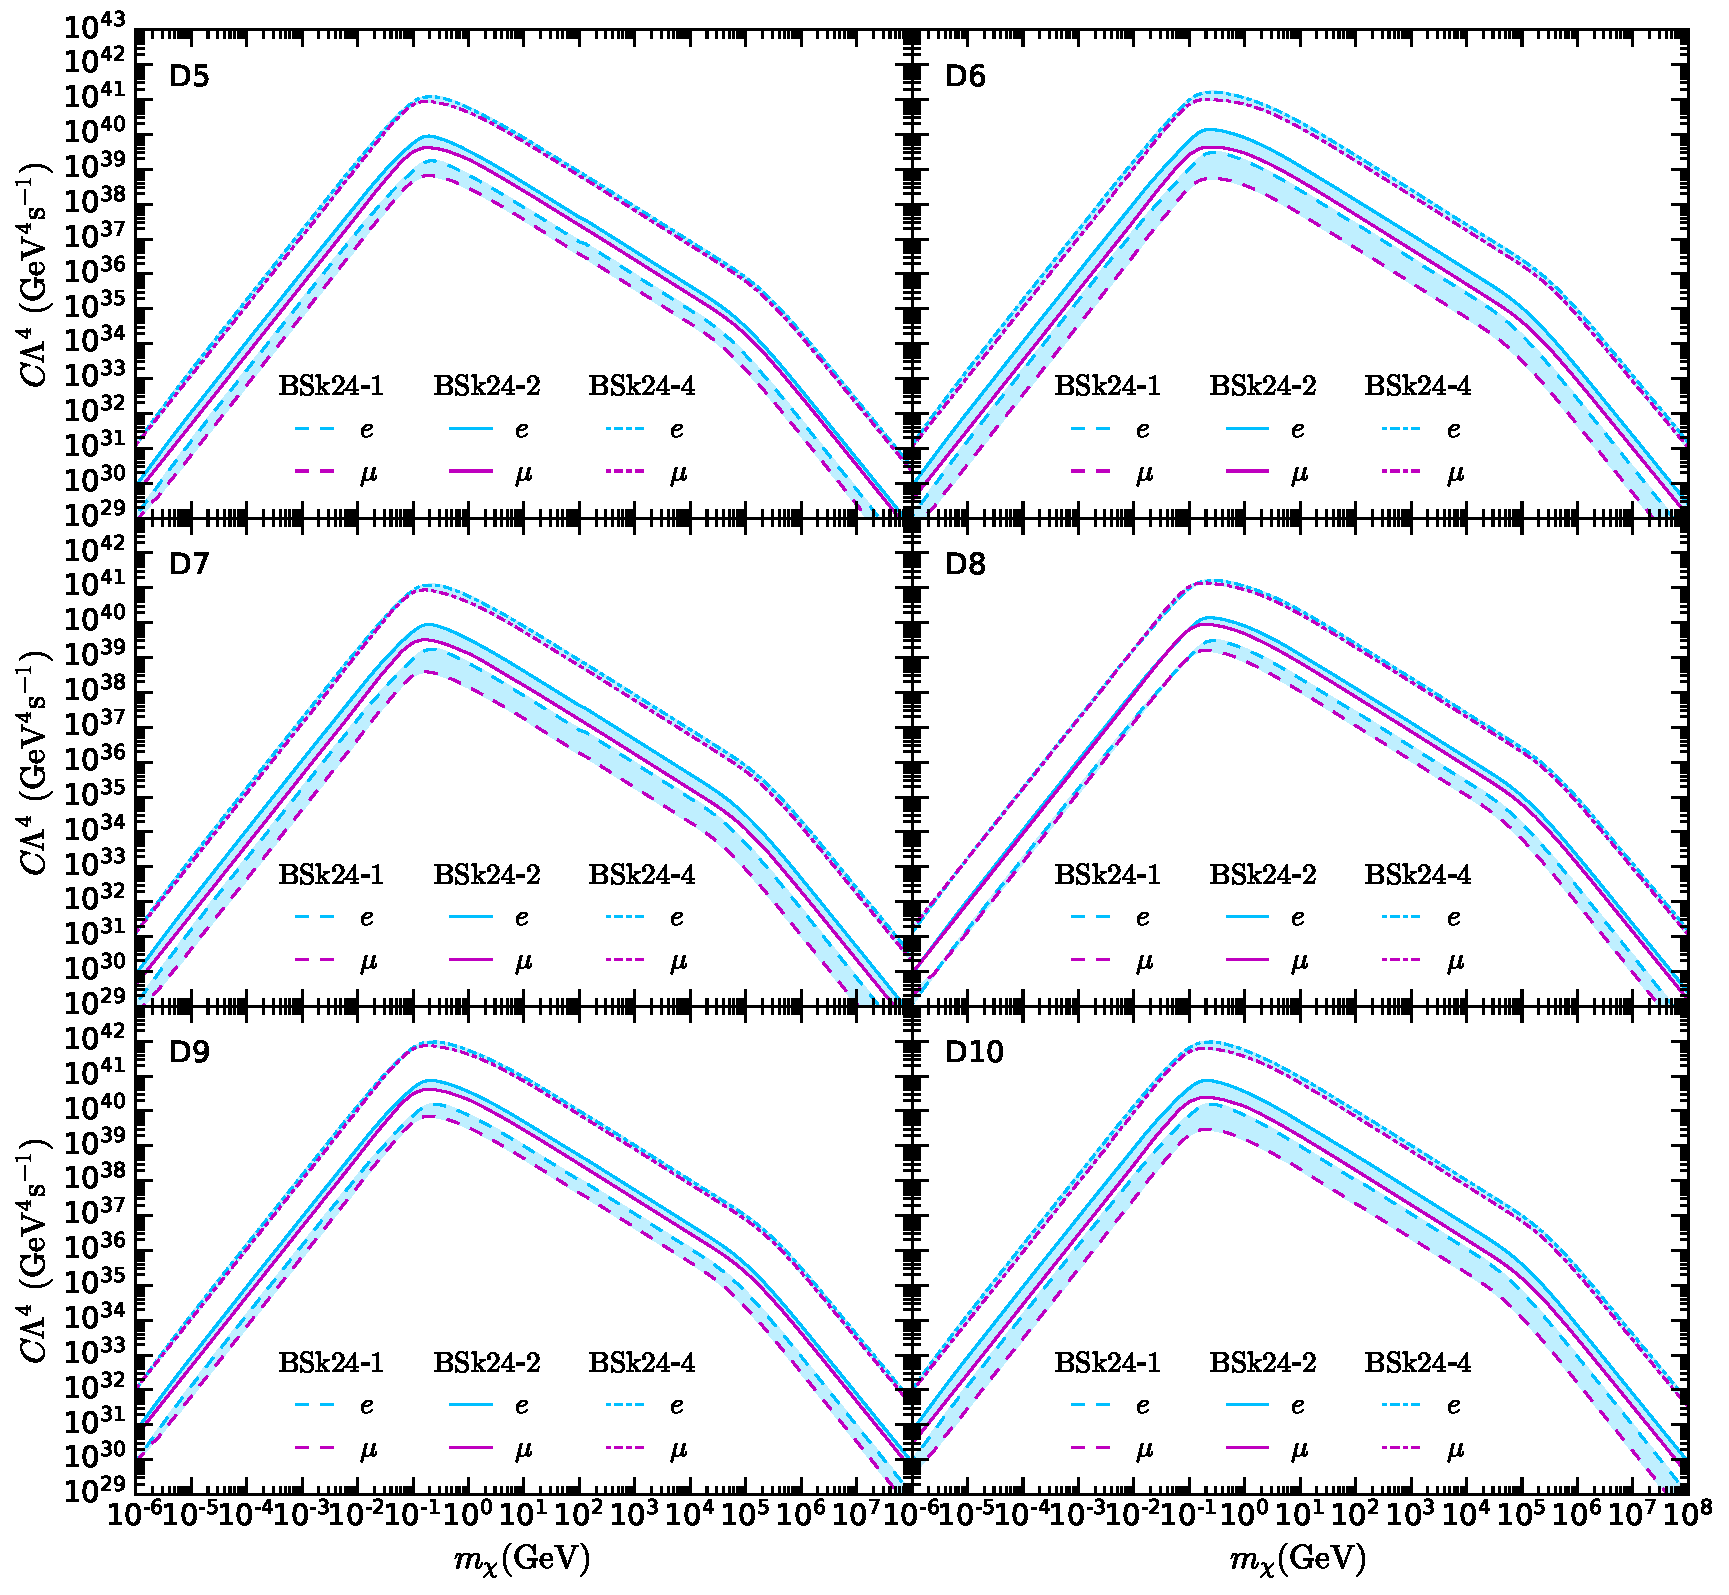
\includegraphics[width=\textwidth]{capture_2/D5_D10_C_mDM_lept.pdf}
    \caption[Capture rate in the optically thin limit for operators D5-D10 as a function of the DM mass $m_\chi$ for electrons (light blue) and muons (magenta) in the NS benchmark models BSk24-1 (dashed), BSk24-2 (solid) and BSk24-4 (dot-dashed).]{Capture rate in the optically thin limit for operators D5-D10 as a function of the DM mass $m_\chi$ for electrons (light blue) and muons (magenta) in the NS benchmark models BSk24-1 (dashed), BSk24-2 (solid) and BSk24-4 (dot-dashed). All capture rates scale as $\Lambda^{-4}$. The shaded regions depict the difference between capture by electrons and muons for the above-mentioned NS models. 
    }
    \label{ch4:fig:capratesD5D10}
    \end{figure}

    

Figs.~\ref{ch4:fig:capratesD1D4} and~\ref{ch4:fig:capratesD5D10} show the results for electron (light blue) and muon (magenta) targets, considering three NS benchmark models: BSk24-1 (dashed, $1\Msun$), BSk24-2 (solid, $1.5\Msun$) and BSk24-4 (dot-dashed, $2.16\Msun$) We assume a nearby NS, located in the Solar neighbourhood, and thus take $\rho_\chi=0.4\GeV\cm^{-3}$, $\vstar=230\km\s^{-1}$ and $v_d=270\km\s^{-1}$.  

\begin{table}[t!bp]
    \centering
    \begin{tabular}{l c c}
    \toprule
    Target & $\mu$ & $e$  \\
    \midrule\midrule
    $m_\ell^*\; (\GeV)$  & $[0.3,3] \times 10^{5}$ & $[0.05,1.7] \times 10^{5}$  \\
    $\sigmathl\; (\cm^2)$ &  $8\times 10^{-44}$ & $3\times 10^{-44}$ \\
    \bottomrule
    \end{tabular} 
    \caption[Typical values of $m_\ell^*$ and $\sigmathl$ for lepton targets. ]{Typical values of $m_\ell^*$ and $\sigmathl$ for lepton targets. 
    The exact value of $\sigmathl$ depends on the DM mass, and the operator. We show here the simplest case of constant matrix element; other operators give similar results. The threshold cross-section is approximately constant in the range $1\GeV\lesssim m_\chi\lesssim m_\ell^*$, and takes larger values outside that range with a $1/m_\chi$ or $m_\chi$ scaling for small and large masses, respectively. }
    \label{ch4:tab:mstarsigma}
    \end{table} 

In these figures, we observe that the capture rate is suppressed due to Pauli blocking when $m_\chi \lesssim m_\ell$. The change of slope at $m_\chi\sim m_\ell^* \sim 10^5\GeV$, observed for both targets, is due to multiple scattering. 
For the operators D5-10 (Fig.~\ref{ch4:fig:capratesD5D10}), whose matrix elements depend explicitly on $s$,  the slope of the capture rate in the three mass regimes are all very similar to one another, while for D1-D4 (Fig.~\ref{ch4:fig:capratesD1D4}), the shape of $C$ is controlled by the power of $t$ that dominates the interaction, which in general is the lowest power \cite{Bell:2020jou_sep_ImprovedTreatmentDark}. 

The exceptions to this are the capture rates for operators D1 and D2 with electron targets, which show a distinctive feature in the region $m_e\lesssim m_\chi\lesssim 100\MeV$ that does not occur for the other operators.  
The capture rate for D1 and D2 is more suppressed in that particular region, similarly to D3 and D4, respectively. This is due to the form of the corresponding matrix elements together with the smallness of the electron mass. Namely, 
D1 and D2 are the only two operators that contain a factor $(t-4 m_\ell^2)$ in their scattering amplitudes, which for electrons means that the lowest power of $t$ in $\Msq$ is multiplied by $m_e^2$, i.e. these terms are suppressed in the $m_e \lesssim m_\chi\lesssim 100\MeV$ range. Consequently, the capture rate in that DM mass region is dominated by the unsuppressed $t$-terms  in $\Msq$, these being $t$  for D1 (as for D3) and $t^2$ for D2 (see Table~\ref{ch1:tab:opers_defn_full}), while below $m_e$ this additional suppression disappears and the capture rate follows the lowest power of $t$ as was originally expected. 

From Fig.~\ref{ch4:fig:capratesD1D4}, we note that for the same cutoff scale $\Lambda$, the muon contribution to the total capture rate for operators D1-D4 surpasses that of the electron by approximately 4 orders of magnitude for most of the DM mass range, and by about 8 orders of magnitude at very low mass for operators D1-D2. This is in part due to the large hierarchy between DM couplings to electrons and muons, which is of order $(\frac{m_\mu}{m_e})^2\sim 10^4$, present in all operators D1-4. The additional suppression seen in D1-2 stems from the ultra-relativistic nature of the electrons discussed above. This leads to the electron matrix element being dominated by terms $\propto t^2$ compared to $t$ for the muons in the mass range $m_e \lesssim m_\chi\lesssim 100\MeV$, resulting in the additional 4 orders of magnitude of suppression.

For operators D5-D10, electrons and muons will have the same strength couplings to DM (see Table~\ref{ch1:tab:opers_defn_full}). However, despite similar couplings and a lower abundance, muons are still able to capture DM at a rate comparable to electrons (see light blue regions in Fig.~\ref{ch4:fig:capratesD5D10}), thanks to their larger mass and lower chemical potential (see Fig.~\ref{ch4:fig:NSradprofs1}, right panels). This means that their interactions with DM are less Pauli suppressed, leading to a larger interaction rate. The small difference between the rates at which electron and muon are able to capture DM particles reduces for heavier NS configurations, e.g. from a factor $\sim5$ (BSk24-1) to $\sim 1.5$ (BSk24-4) for D6 and D10; see the light blue shaded regions in Fig.~\ref{ch4:fig:capratesD5D10}. This is due to the muon abundance increasing in heavier NSs.



It is also worth noting that different EoS assumptions can lead to variations in the capture rate for electron targets of at least two orders of magnitude in the Pauli suppressed region and $\sim 2.5$ orders of magnitude in the large DM mass regime (compare dashed with dot-dashed light blue lines). For muons, the effect is even larger, with capture rate variations from $\sim {\cal O}(5\times 10^2)$ for low DM mass to $\sim {\cal O}(2\times 10^3)$ for heavy DM, when comparing the lightest and most massive NS configurations of the BSk24 family. For the operators D2 and D4, these variations are even more pronounced for both electrons and muons and can reach  $\sim {\cal O}(5\times 10^3)$ and  $\sim {\cal O}(5\times 10^4)$, respectively for very large DM masses. 


\begin{figure}
    \centering
    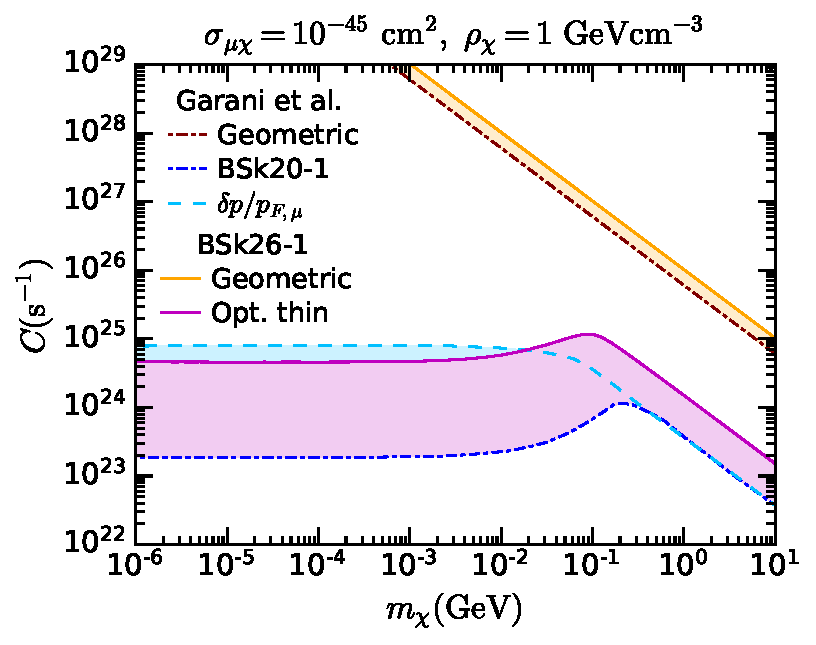
\includegraphics[width=.7\textwidth]{capture_2/capture_rate_n0_comp_muons.pdf}
    \caption[Capture rate in the optically thin limit for muon targets as a function of the DM mass for a constant cross-section, $\sigma_{\mu\chi}=10^{-45}\cm^2$,  $\rho_\chi=1\GeV\cm^{-3}$ and BSk26 functional for $\Mstar\simeq1.52\Msun$ and $\Rstar\simeq11.6\km$ denoted as BSk26-1. Capture rate calculations from Ref.~\cite{Garani:2018kkd_may_NewAnalysisNeutron}.]{Capture rate in the optically thin limit for muon targets  (magenta) and geometric (orange) limit as a function of the DM mass for constant cross-section $\sigma_{\mu\chi}=10^{-45}\cm^2$,  $\rho_\chi=1\GeV\cm^{-3}$ and BSk26 functional for $\Mstar\simeq1.52\Msun$ and $\Rstar\simeq11.6\km$ denoted as BSk26-1. Capture rate calculations from Ref.~\cite{Garani:2018kkd_may_NewAnalysisNeutron} for a NS configuration with EoS BSk20-1~\cite{Potekhin:2013qqa_Analyticalrepresentationsunified} equivalent to BSk26-1, are shown for comparison. 
    }
    \label{ch4:fig:Cratecomp}
\end{figure}
  

The DM capture rate for muon targets was calculated in Ref.~\cite{Garani:2018kkd_may_NewAnalysisNeutron}, for constant cross-section and light DM, $m_\chi\leq10\GeV$. That calculation accounts for the NS internal structure and Pauli blocking, but neglects general relativity (GR) corrections and assumes that muons are non-relativistic. 
As outlined in Section~\ref{ch3:subsec:captureintermediate}, to compare our capture rate calculation with that of Ref.~\cite{Garani:2018kkd_may_NewAnalysisNeutron}  we select a NS model that matches that of Fig.~12 of Ref.~\cite{Garani:2018kkd_may_NewAnalysisNeutron}, namely Model A (BSk20-1):  $\Mstar\simeq1.52\Msun$, $\Rstar\simeq11.6\km$. This new benchmark model is denoted as BSk26-1.  

In Fig.~\ref{ch4:fig:Cratecomp}, we compare both capture rate calculations for  $\sigma_{\mu\chi}=10^{-45}\cm^2$ and the same assumptions about $\rho_\chi$, $v_\star$ and $v_d$ as in Ref.~\cite{Garani:2018kkd_may_NewAnalysisNeutron}. Comparing the geometric limit, Eq.~\ref{ch3:eq:capturegeom}  (solid orange), which properly accounts for gravitational focusing in NSs, with the non-relativistic computation in Ref.~\cite{Garani:2018kkd_may_NewAnalysisNeutron} (dot-dashed brown), we observe a $\sim 67 \%$ enhancement, due to the $1/B(\Rstar)$ factor that encodes GR corrections~\cite{Goldman:1989nd_WeaklyInteractingMassive,Kouvaris:2007ay_WIMPAnnihilationCooling}. 
In the region not affected by Pauli blocking, $m_\chi \gtrsim m_\mu$, our calculation in the optical thin limit (solid magenta) exceeds that of Ref.~\cite{Garani:2018kkd_may_NewAnalysisNeutron} (dot-dashed blue) by a factor of $\sim 4$, which increases as we move to the Pauli suppressed region where our computation is more than one order of magnitude higher. Unlike Ref.~\cite{Garani:2018kkd_may_NewAnalysisNeutron}, our formalism incorporates GR corrections and made use of relativistic kinematics. We also show in dashed light blue, an estimation of the capture rate using the approximation $\delta p/p_{F,\mu}\sim m_\chi v_{esc}/p_{F,\mu}$  for $m_\chi < m_\mu$~\cite{McDermott:2011jp_ConstraintsScalarAsymmetric}, where $p_{F,\mu}$ is the muon Fermi momentum and $v_{esc}$ is the escape velocity. This approximation overestimates the capture rate by a factor of approximately 2 in the Pauli blocked region below 10 MeV and underestimates it in the region of larger DM masses. 





%%%%%%%%%%%%%%%%%%%%%%%%%%%%%%%%%%%%%%%%%%%%%%%%%%%%%%%%%%%%%%%%%%%%%%%%%%%%%%%%%%%%
\subsection{Finite Temperature Effects and Evaporation}
\label{ch4:subsec:finite_temp_NS}
%%%%%%%%%%%%%%%%%%%%%%%%%%%%%%%%%%%%%%%%%%%%%%%%%%%%%%%%%%%%%%%%%%%%%%%%%%%%%%%%%%%%



In Section~\ref{ch4:subsec:caprateresults}, we have restricted our computation of the capture rates to the DM mass range $m_\chi\in[1\keV,10^8\GeV]$. While the upper limit on this mass range is somewhat arbitrary, primarily limited by the increasing numerical tax of calculating Eq.~\ref{ch3:eq:capturesimplelargem}, the lower bound comes from working in the zero-temperature approximation, $\Tstar \rightarrow 0$. This approximation is valid for DM masses $\mchi \gg\Tstar$, which for a $10^3\K$ star requires $\mchi \gg 90$ meV.

For DM masses $m_\chi\lesssim \mathcal{O}(10)\Tstar$, thermal effects begin to play an important role in the capture rate, significantly boosting the rate in this low mass range~\cite{Garani:2018kkd_may_NewAnalysisNeutron}. Consequently, the complete Fermi-Dirac distributions should be used in Eqs.~\ref{ch3:eq:scattrate} and~\ref{ch3:eq:int_rate_capture_full}. To illustrate the effect of the NS temperature,  we show in Fig.~\ref{ch4:fig:CfiniteT_e} the ratio of the capture rate in a NS with 
$\Tstar=10^5\K\simeq8.6\eV$ to the corresponding capture rate in the $\Tstar\rightarrow0$ limit, assuming scattering on electrons, the targets for which this effect is most relevant. 

From this figure, we immediately notice that the ratio starts to depart from  $1$ at $m_\chi\sim100\eV\sim 10T_\star$ for all operators. Operators whose matrix element depends on higher powers of the exchanged momentum  $t$ feature a larger increment in the capture rate due to finite temperature. In fact, the operator D4 ($|\overline{\mathcal{M}}|^2\propto t^2$) receives the largest correction, followed by D2-D3 (whose $|\overline{\mathcal{M}}|^2$ is a linear combination of $t^1,t^2$), then D1 ($|\overline{\mathcal{M}}|^2$ is a linear combination of $t^0,t^1,t^2$) and finally by  D5-D10 (whose $|\overline{\mathcal{M}}|^2$ include all powers of the kind $t^n s^m$).

\begin{figure}[t!bp]
    \centering
    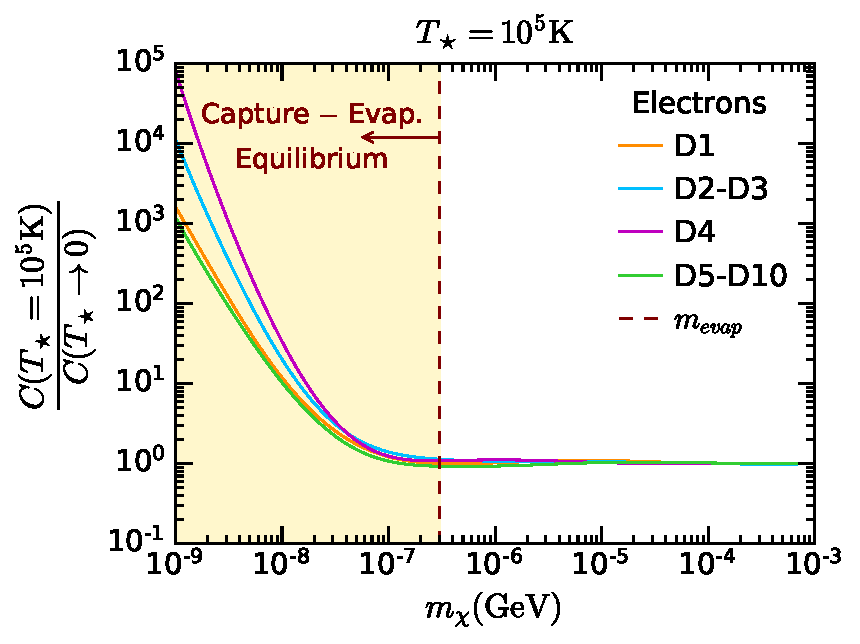
\includegraphics[width=0.7\textwidth]{capture_2/R_CT_mdm_10_5K_D1_D10_e.pdf}
    \caption[Finite temperature effects on the capture rate for electron targets, assuming the NS model BSk24-2.]{Finite temperature effects on the capture rate for electron targets, assuming the NS model BSk24-2. The DM mass range where capture and evaporation are expected to be in equilibrium is shaded in yellow. The dashed brown line corresponds to the evaporation mass.}
    \label{ch4:fig:CfiniteT_e}
\end{figure}


In the very light DM regime, there is another that needs to be accounted for: evaporation. This occurs when the dark matter up-scatters to a state where the final DM kinetic energy is larger than the energy required to escape the star, and hence DM particles are expelled. Thus, as opposed to capture, evaporation drains energy from the star. 
To estimate the evaporation rate, we convolve the DM distribution within the star, with the interaction rate for up-scattering, $\Gamma^-_\mathrm{up}(E_\chi, \Tstar)$, retaining the temperature dependence.

Assuming the DM distribution to be isothermal with temperature $T_\chi=\Tstar$, we have 
\begin{align}
n_\chi^\mathrm{iso}(r,E_\chi) &= \frac{n_c}{1+e^{\frac{E_\chi-m_\chi\left(\frac{1}{\sqrt{B(r)}}-1\right)}{\Tstar}}} \\
& \simeq \frac{ \exp\left[-\frac{E_\chi-m_\chi\left(\frac{1}{\sqrt{B(r)}}-1\right)}{\Tstar}\right]}{4\pi \int_0^{\Rstar} dr r^2  \int_0^{m_\chi\left(\frac{1}{\sqrt{B(r)}}-1\right)} dE_\chi \exp \left[{-\frac{E_\chi-m_\chi\left(\frac{1}{\sqrt{B(r)}}-1\right)}{\Tstar}}\right]}, 
\end{align}
where $n_c$ is a normalisation constant such that the total number of DM particles is $N_\chi = \int d^3r\int dE_\chi\;n_\chi^\mathrm{iso}(E_\chi, r)$. The interaction rate for up-scattering, $\Gamma^-_\mathrm{up}(E_\chi, \Tstar)$ can be related to the down-scattering rate through
\begin{equation}
\frac{d\Gamma^-_\mathrm{up}}{dq_0}\left(E_\chi, q_0,\Tstar\right) = -\frac{e^{q_0/\Tstar}}{1-e^{q_0/\Tstar}} \dfrac{d\Gamma^-}{dq_0}\left(E_\chi, q_0\right),\quad q_0<0,
\label{ch4:eq:upscattintrate}
\end{equation}
where $\tfrac{d\Gamma^-}{dq_0}$ is the differential interaction rate in the $\Tstar\rightarrow 0$ approximation derived in Appendix~\ref{app:subsec:down_scatter_derivation}, with the full derivation of Eq.~\ref{ch4:eq:upscattintrate} in Appendix~\ref{app:subsec:up_scatter_derivation}. 

The evaporation rate then reads
\small
\begin{align}
E &\simeq 4\pi \int_0^{\Rstar} dr r^2 \int_0^{m_\chi\left(\frac{1}{\sqrt{B(r)}}-1\right)}dE_\chi n_\chi^\mathrm{iso}(r,E_\chi) \int_{-\infty}^{-q_0^\mathrm{min}} dq_0 \frac{d\Gamma^-_\mathrm{up}}{dq_0}\left(q_0,\Tstar\right), \\
q_0^\mathrm{min} & = m_\chi\left(\frac{1}{\sqrt{B(r)}}-1\right)-E_\chi,
\label{ch4:eq:evaprate}
\end{align}
\normalsize
where $q_0^\mathrm{min}$ is the minimum energy the DM needs to gain to be ejected from the star.
When the DM distribution is concentrated very close to the centre of the star, this expression can be approximated by
\begin{equation}
E \sim  \frac{ m_\chi m_\ell^2\sigma_{\ell\chi}}{4\pi^2} \left(\frac{1}{\sqrt{B(0)}}-1\right)^2  \exp\left[{-\frac{m_\chi}{\Tstar}}\left(\frac{1}{\sqrt{B(0)}}-1\right)\right]. \end{equation}
% 
The rate at which DM particles accumulate in NSs is then given by
\begin{equation}
\dfrac{dN_\chi}{dt} = C- E N_\chi,
\end{equation}
assuming that DM annihilation is negligible. The solution of this equation is 
\begin{equation}
N_\chi(\tstar) = C \, \tstar \left( \frac{ 1-e^{-E \, \tstar}}{E \, \tstar} \right),   
\end{equation}
where $\tstar$ is the age of the NS. The term in brackets quantifies the depletion of the number of capture DM particles due to the evaporation process. This factor will be of order 1 unless $E(m_\chi) \, t_\star \gtrsim {\cal O}(1)$. Therefore, we will define the evaporation mass as the DM mass for which the previous relation holds, i.e.  $E(m_\mathrm{evap}) t_\star \sim 1$. 
For DM masses below this threshold, $m_\chi \lesssim m_\mathrm{evap}$, the capture and evaporation processes are in equilibrium with each other. In that limit, the net energy exchange in the star due to the combined effects of DM capture and evaporation would be negligible, and hence we would be unable to constrain DM interactions using the NS temperature as a probe.


Using Eq.~\ref{ch4:eq:evaprate}, we find the evaporation mass to be of order $m_\mathrm{evap}\sim\mathcal{O}(100\Tstar)$ for all scattering targets in old NSs with $\tstar\sim{\cal O}(10 \Gyr)$. For instance, for $\Tstar=10^5\K$ and electron targets, we obtain $m^e_\mathrm{evap}\simeq 300\eV$. 
The region in Fig.~\ref{ch4:fig:CfiniteT_e} for which capture and evaporation are in equilibrium is shaded in yellow, with the evaporation mass indicated by the dashed brown line. From this, we can see that the finite temperature effects on the capture rate come become importatnt for masses below the evaporation mass, for all operators we consider. Hence, when calculating the capture rate while aiming to constrain DM interactions, finite temperature effects can be safely neglected.



%%%%%%%%%%%%%%%%%%%%%%%%%%%%%%%%%%%%%%%%%%%%%%%%%%%%%%%%%%%%%%%%%%%%%%%%%%%%%%%%%%%%
%%%%%%%%%%%%%%%%%%%%%%%%%%%%%%%%%%%%%%%%%%%%%%%%%%%%%%%%%%%%%%%%%%%%%%%%%%%%%%%%%%%%
\subsection{Results}
\label{ch4:subsec:results_NS}
%%%%%%%%%%%%%%%%%%%%%%%%%%%%%%%%%%%%%%%%%%%%%%%%%%%%%%%%%%%%%%%%%%%%%%%%%%%%%%%%%%%%
%%%%%%%%%%%%%%%%%%%%%%%%%%%%%%%%%%%%%%%%%%%%%%%%%%%%%%%%%%%%%%%%%%%%%%%%%%%%%%%%%%%%

%%%%%%%%%%%%%%%%%%%%%%%%%%%%%%%%%%%%%%%%%%%%%%%%%%%%%%%%%%%%%%%%%%%%%%%%%%%%%%%%%%%%
\subsubsection{Threshold Cross-Sections}
\label{ch4:subsubsec:thxs}
%%%%%%%%%%%%%%%%%%%%%%%%%%%%%%%%%%%%%%%%%%%%%%%%%%%%%%%%%%%%%%%%%%%%%%%%%%%%%%%%%%%%

In Section~\ref{ch3:subsec:geom_lim_threshold_xs}, we defined the threshold cross-section, $\sigmathl$, as the cross-section for which the capture rate, $C(\sigma(\Lambda),m_\chi)$, calculated in the optically thin regime becomes equal to the geometric limit, $C_\mathrm{geom}$. 
The threshold cross-section restricts the NS sensitivity to DM-target interactions since for $\sigma\ge\sigmathl$ the capture rate saturates to the geometric limit $C_\mathrm{geom}$. 



In Fig.~\ref{ch4:fig:sigmathe}, we show the threshold cross-sections for lepton targets, electrons and muons, and compare them with existing direct detection limits and expected sensitivities of future experiments. The neutrino floor for electron recoil experiments for silicon targets~\cite{Essig:2018tss_Solarneutrinossignal} is shown as a shaded yellow region.
The solid light blue and magenta lines correspond to the value of $\sigma_{th}$ for electrons and muons respectively, calculated using the NS model BSk24-2  ($1.5 M_\odot$), while the shaded bands in light blue and magenta denote the expected range for $\sigma_{th}$ for the two different targets, obtained by varying the NS configuration along the BSk24 family. 
 BSk24-1 ($1M_\odot$) gives the upper bound on $\sigmath$ and BSk24-4 ($2.16 M_\odot$) the lower bound. 
Note that the variation in $\sigmath$ due to the NS EoS increases with the DM mass and for muons goes from about one order of magnitude in the low mass range, to two orders of magnitude in the multiple scattering region. For electrons, this effect is slightly less pronounced.


    
All the limits for existing experiments are orders of magnitude weaker than the expected NS reach, with only the future DAMIC-M~\cite{Essig:2015cda_DirectdetectionsubGeV} (dashed brown line) expected to surpass NS electron scattering sensitivity and approach that of muons, in the DM mass range  $3\MeV\lesssim m_\chi\lesssim 30\MeV$. Moreover, NS sensitivity to DM interactions with lepton targets is expected to be well below the neutrino floor for $m_\chi\gtrsim 100\MeV$ and, in the case of muons, even for $m_\chi\lesssim 1\MeV$. 

\begin{figure}[t!bp]
    \centering
    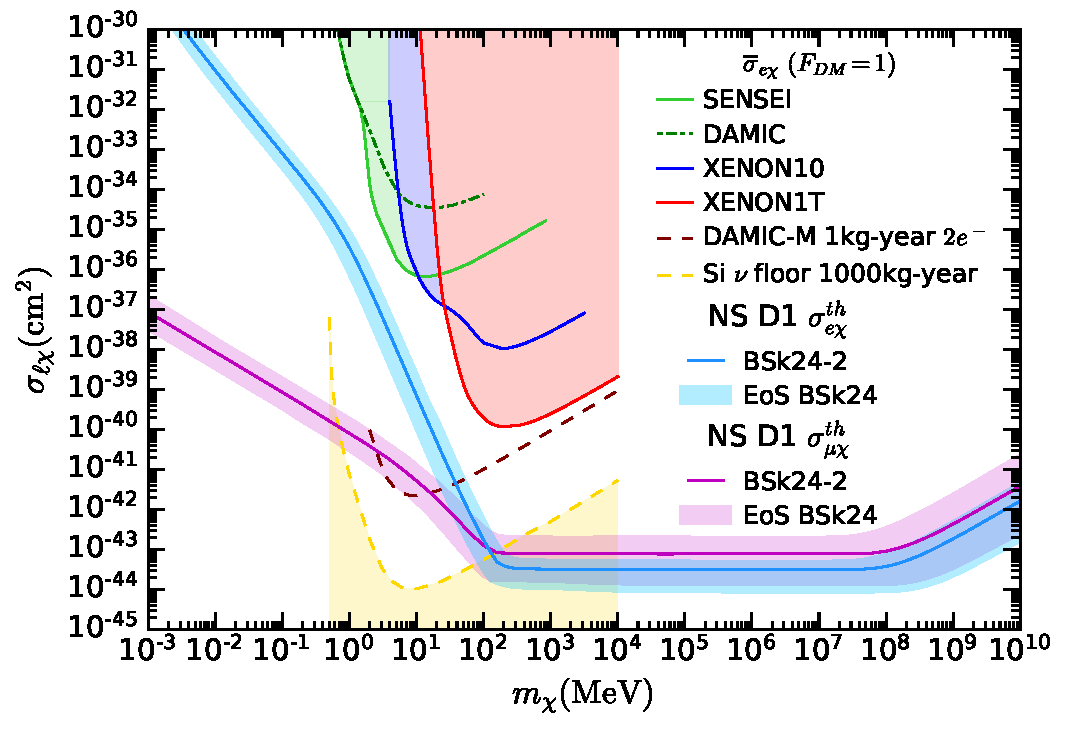
\includegraphics[width=0.49\textwidth]{capture_2/DD_NS_leptons.pdf}
    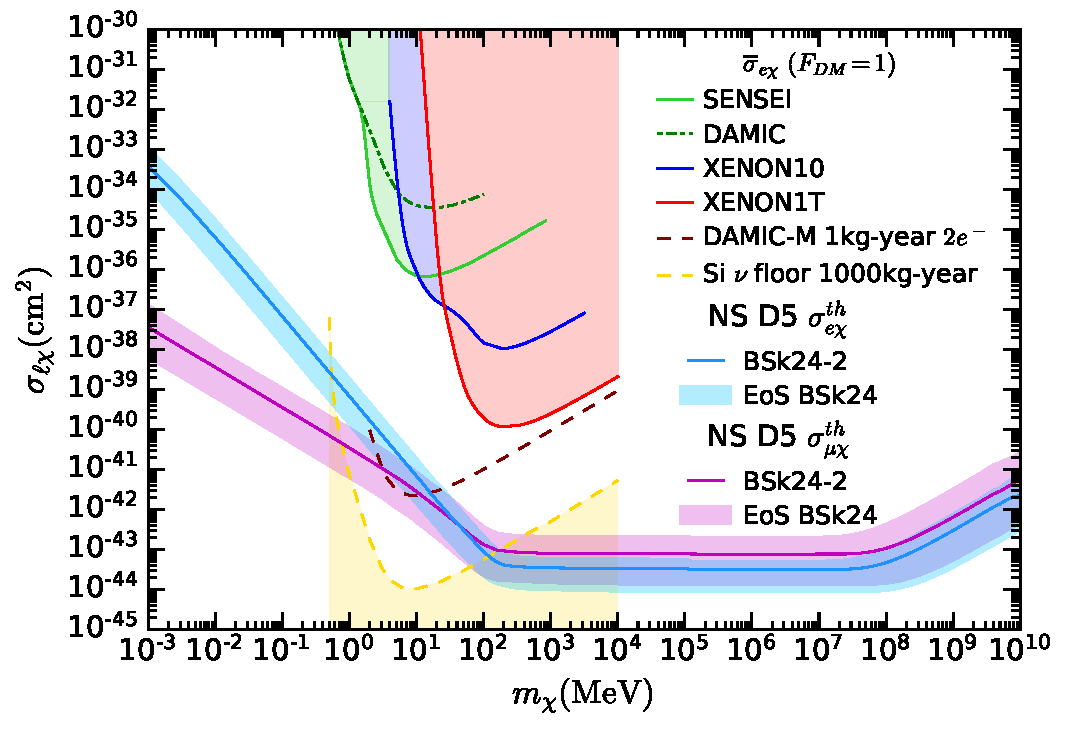
\includegraphics[width=0.49\textwidth]{capture_2/DD_NS_leptons_D5.pdf}
    \caption[DM-lepton threshold cross-section for operators D1 (left) and D5 (right) for the EoS BSk24.]{DM-lepton threshold cross-section for operators D1 (left) and D5 (right) for the EoS BSk24. The solid blue (electron) and magenta (muon) lines represent $\sigmath$, are computed assuming the NS model BSk24-2, while the shaded bands represent the expected range due to variation of the EoS. For comparison, we show leading electron recoil bounds for heavy mediators from SENSEI~\cite{SENSEI:2020dpa_SENSEIDirectdetectionresults}, DAMIC~\cite{DAMIC:2019dcn_Constraintslightdark}, Xenon10~\cite{Essig:2017kqs_Newconstraintsprospects}, Xenon1T~\cite{XENON:2019gfn_Lightdarkmatter}, projected sensitivities from DAMIC-M~\cite{Essig:2015cda_DirectdetectionsubGeV} as well as the neutrino floor for silicon detectors~\cite{Essig:2018tss_Solarneutrinossignal}.}
        \label{ch4:fig:sigmathe}
\end{figure}

Note that NSs have a better sensitivity to vector-vector interactions (operator D5, see right panel) than scalar-scalar interactions (operator D1, see left panel) in the low DM regime for both leptonic targets, and especially for electrons. As discussed in Section~\ref{ch4:subsec:caprateresults}, there is an additional suppression in the capture rates for scalar operators, which stems from an $m_e^2 \, t$ term in their scattering amplitudes. 

Similar threshold cross-sections can be estimated for the remaining operators.  Operators with s-dependent matrix elements (D6-D10) have  $\sigmath$ that behave like that of D5 for both electrons and muons. D2 presents the same features as D1 in the sub-GeV regime for electrons due to the similar shape of their capture rates (see Fig.~\ref{ch4:fig:capratesD1D4}) and D3-D4 show steeper slopes in the $m_\chi\lesssim m_e$ region with respect to D1-D2, due to the capture rate dependence on higher powers of $t$. 



%%%%%%%%%%%%%%%%%%%%%%%%%%%%%%%%%%%%%%%%%%%%%%%%%%
\subsubsection{Comparison with Literature}
\label{ch4:subsubsec:literature_comp_NS}
%%%%%%%%%%%%%%%%%%%%%%%%%%%%%%%%%%%%%%%%%%%%%%%%%%

We now compare our calculations for the capture rates and resulting reach in the EFT cutoff $\Lambda$ for operators D1 and D5 to those presented in Refs.~\cite{Joglekar:2019vzy_sep_Relativisticcapturedark,Joglekar:2020liw_Darkkineticheating}\footnote{Note that the Yukawa couplings for scalar and pseudoscalar operators in Refs.~\cite{Joglekar:2019vzy_sep_Relativisticcapturedark,Joglekar:2020liw_Darkkineticheating} are embedded into the cutoff scale $\Lambda$.}.
The formalism in Refs.~\cite{Joglekar:2019vzy_sep_Relativisticcapturedark,Joglekar:2020liw_Darkkineticheating} is valid for relativistic and non-relativistic targets in a broad mass range; however, several simplifying assumptions were made in those refs, while er adopt a more accurate treatment. Namely, they do not account for the DM velocity distribution far from the star, nor do they incorporate the internal structure of the NS. Instead, constant chemical potentials and particle abundances that have been averaged over the core volume are used. These quantities correspond to the NS model BSk24-2 and were calculated in Ref.~\cite{Bell:2019pyc_jun_CaptureLeptophilicDark}. 



\begin{figure}[t!bp]
    \centering
    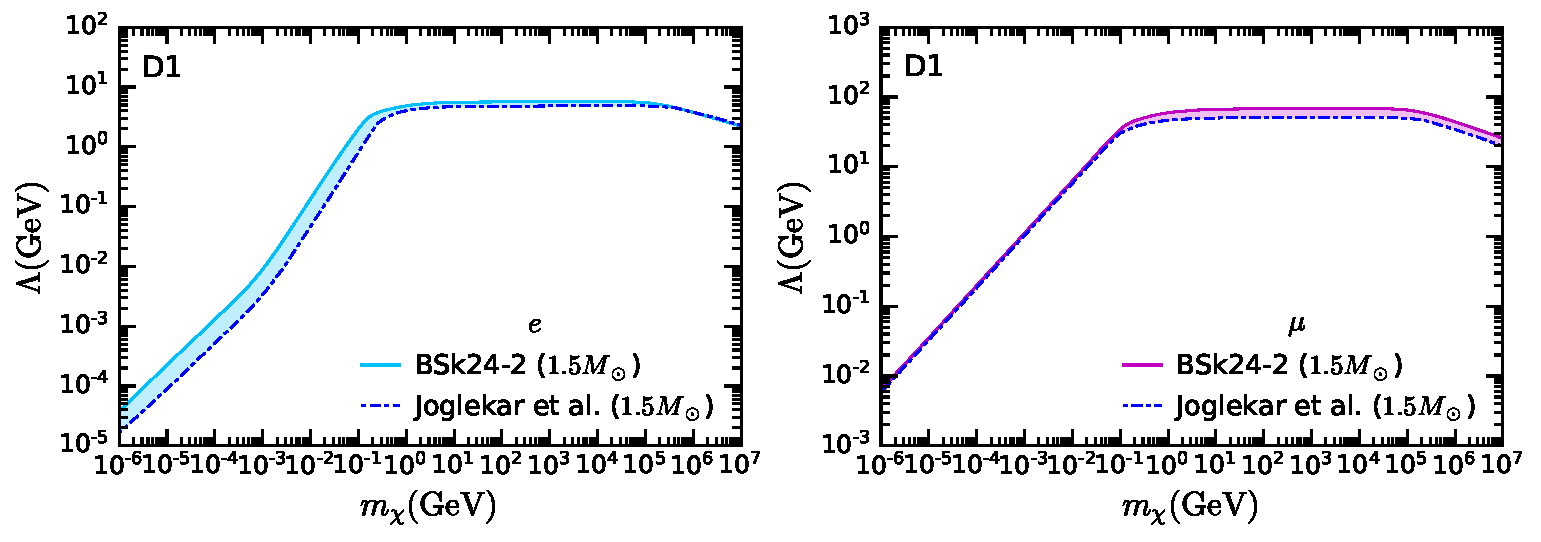
\includegraphics[width=\textwidth]{capture_2/D1_Lambda_mdm_leptons.pdf}\\
    \vspace*{-0.5em}    
    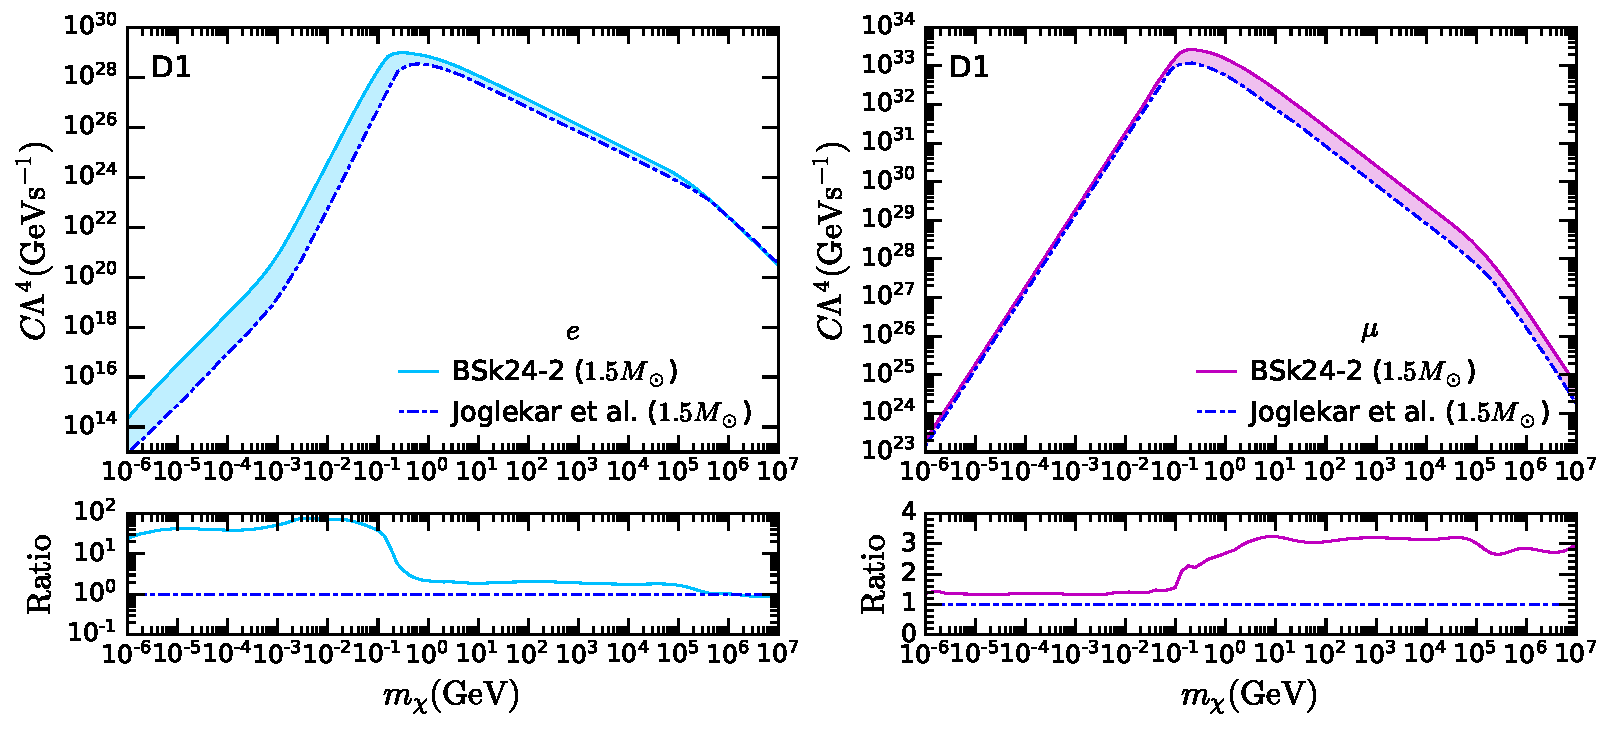
\includegraphics[width=\textwidth]{capture_2/D1_C_mdm_leptons.pdf}     
    \caption[Comparison of the reach in $\Lambda$ for D1 with the approach of Ref.~\cite{Joglekar:2020liw_Darkkineticheating}. ]{Comparison of the reach in $\Lambda$ for D1 with the approach of Ref.~\cite{Joglekar:2020liw_Darkkineticheating}. The shaded regions denote the difference in $\Lambda$ (top) and $C\Lambda^4$ (middle) between the two approaches and their ratio is shown in the bottom panels.}
    \label{ch4:fig:D1_Lambda_mdm}
\end{figure}


    
In the top panels of Figs.~\ref{ch4:fig:D1_Lambda_mdm} and~\ref{ch4:fig:D5_Lambda_mdm}, we compare the reach in $\Lambda$ for DM-lepton scattering cross-sections in Refs.~\cite{Joglekar:2019vzy_sep_Relativisticcapturedark,Joglekar:2020liw_Darkkineticheating} with the cutoff scale we obtain for the maximum capture rate, $C(\Lambda,m_\chi)=C_\mathrm{geom}$. 
Our results differ the most for electron targets in the Pauli suppressed region, by a factor of $\sim 2.5$, and we find Pauli blocking is active at a slightly lighter DM mass. This arises from our use of the full radial profiles for the NS input parameters, and that light DM particles whose interactions are subject to Pauli blocking are captured closer to the surface~\cite{Bell:2020jou_sep_ImprovedTreatmentDark}. The discrepancy is reduced to a factor of  $\sim 1.25$ in the intermediate mass region, and there is almost no difference in the large mass regime. For muons, we find a $\Lambda$ that is, on average, a factor $\sim 1.33$ greater than that of Refs.~\cite{Joglekar:2019vzy_sep_Relativisticcapturedark,Joglekar:2020liw_Darkkineticheating} along the whole DM mass range for D5,  and is in almost perfect agreement in the $m_\chi\lesssim m_\mu$ region for D1. 


\begin{figure}[t!bp]
    \centering
    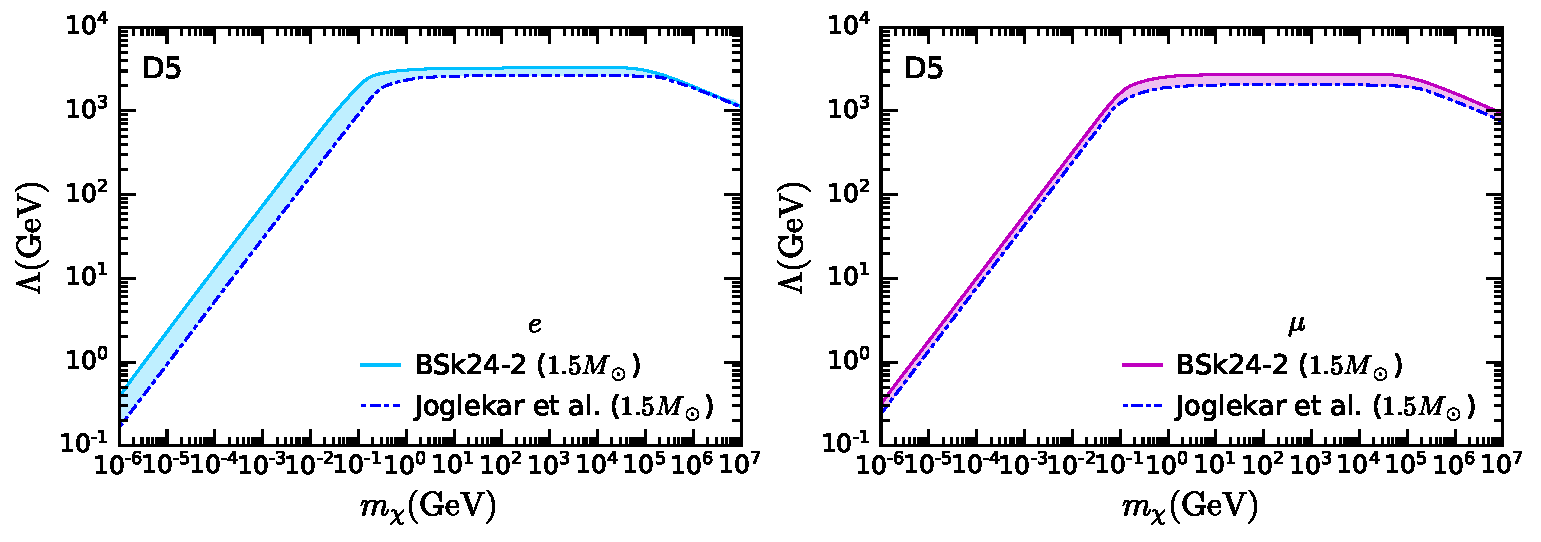
\includegraphics[width=\textwidth]{capture_2/D5_Lambda_mdm_leptons.pdf}\\
    \vspace*{-0.5em}
    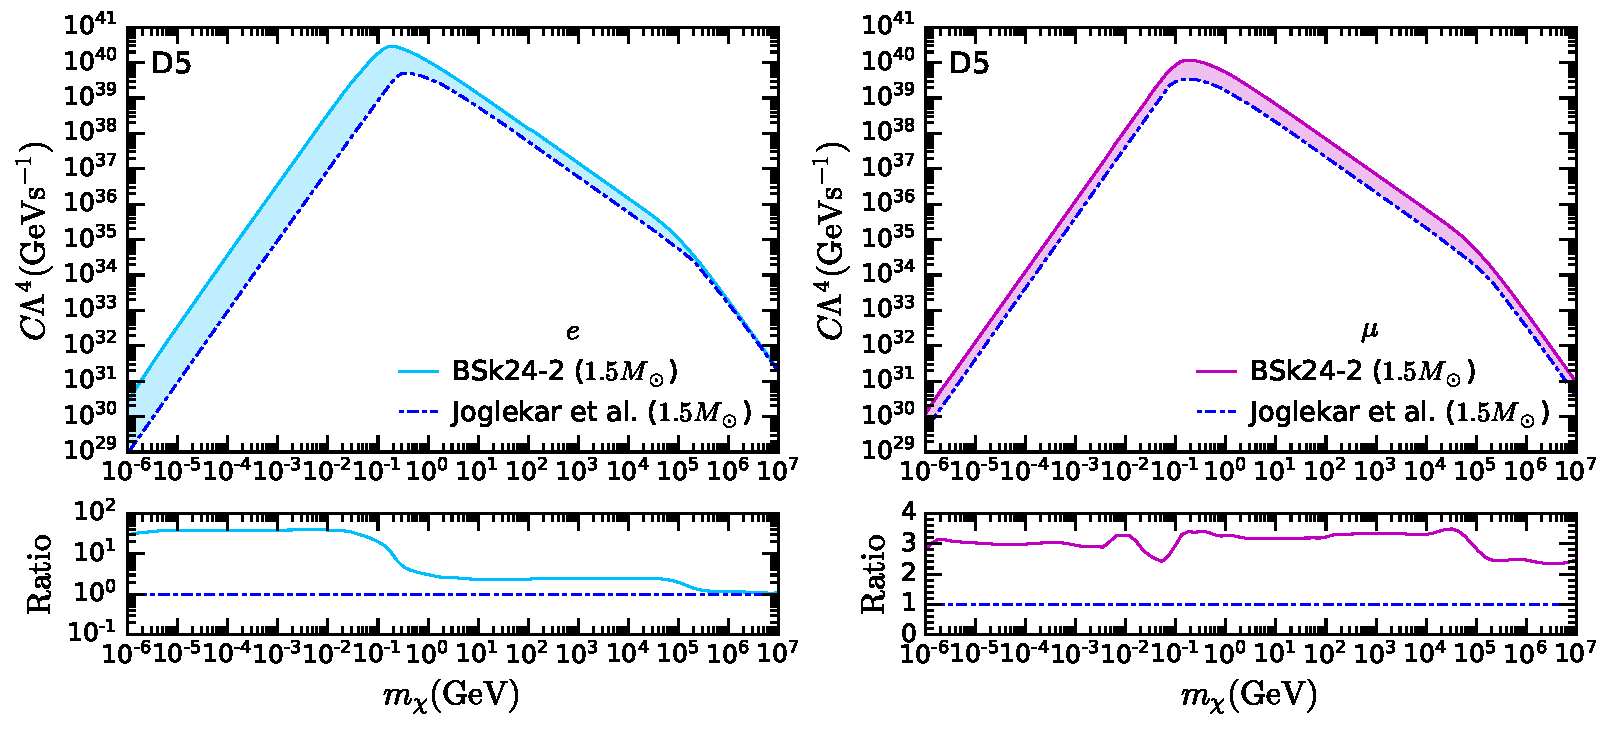
\includegraphics[width=\textwidth]{capture_2/D5_C_mdm_leptons.pdf}    
    \caption{Same as Fig.~\ref{ch4:fig:D1_Lambda_mdm} but for the vector operator D5.}
    \label{ch4:fig:D5_Lambda_mdm}
\end{figure}


In the middle panels of Figs.~\ref{ch4:fig:D1_Lambda_mdm} and~\ref{ch4:fig:D5_Lambda_mdm} we show how these small differences in the two approaches translate to differences in the capture rate, comparing $C \Lambda^4 = \Lambda^4 C_\mathrm{geom}$  obtained with the two formalisms. Since the geometric limit of the capture rate is not defined in Refs.~\cite{Joglekar:2019vzy_sep_Relativisticcapturedark,Joglekar:2020liw_Darkkineticheating}, we use a definition similar to Eq.~\ref{ch3:eq:capturegeom} that is compliant with the assumptions made by these authors. For electron scattering, we see that the formalism that does not account for the NS internal structure underestimates the capture rate in the region affected by Pauli blocking by a factor $\sim 40$ (bottom LH panels of Figs.~\ref{ch4:fig:D1_Lambda_mdm} and ~\ref{ch4:fig:D5_Lambda_mdm}). This difference is slightly larger in the region where the Pauli suppression is stronger, becoming almost a factor of $\sim 100$ for D1 in the range $m_e\lesssim m_\chi \lesssim 100\MeV$. For muons, the difference between the two approaches is less pronounced, with a maximum ratio of $\sim 3.5$ for both operators.



%%%%%%%%%%%%%%%%%%%%%%%%%%%%%%%%%%%%%%%%%%%
%%%%%%%%%%%%%%%%%%%%%%%%%%%%%%%%%%%%%%%%%%%%%%%%%%%%%%%%%%%%%%%%%%%%%%%%%%%%%%%%%%%%
%%%%%%%%%%%%%%%%%%%%%%%%%%%%%%%%%%%%%%%%%%%%%%%%%%%%%%%%%%%%%%%%%%%%%%%%%%%%%%%%%%%%
\section{Capture from Electrons in White Dwarfs}
\label{ch4:sec:capture_WDs}
%%%%%%%%%%%%%%%%%%%%%%%%%%%%%%%%%%%%%%%%%%%%%%%%%%%%%%%%%%%%%%%%%%%%%%%%%%%%%%%%%%%%
%%%%%%%%%%%%%%%%%%%%%%%%%%%%%%%%%%%%%%%%%%%%%%%%%%%%%%%%%%%%%%%%%%%%%%%%%%%%%%%%%%%%

We now turn our attention to DM capture in white dwarfs, where the degenerate electrons preventing these stars from gravitational collapse are a perfect candidate for the capture formalism we have constructed. Not only are the electrons extremely degenerate, with chemical potentials $\kinFe \gg m_e$ in some stars, but they can also be ultra-relativistic. As the gravitational fields of WDs are significantly weaker than those of NSs, the incoming DM does not get boosted to relativistic velocities in this case. This leads to the scattering interactions taking place in an interesting kinematic regime, as we are dealing with non-relativistic DM scattering off ultra-relativistic electrons.
% We thus adopt the formalism developed in Refs.~\cite{Bell:2020jou_sep_ImprovedTreatmentDark,Bell:2020lmm_mar_ImprovedTreatmentDark} for the case of DM capture in neutron stars, which includes the effects mentioned above, uses relativistic kinematics and also considers GR corrections\footnote{For WDs, these corrections turn out to be rather minor due to their significantly weaker gravitational fields compared to NSs.}. 


%%%%%%%%%%%%%%%%%%%%%%%%%%%%%%%%%%%%%
%%%%%%%%%%%%%%%%%%%%%%%%%%%%%%%%%%%%%
\subsection{White Dwarf Refresher}
\label{ch4:subsec:WD_refresh}
%%%%%%%%%%%%%%%%%%%%%%%%%%%%%%%%%%%%%
%%%%%%%%%%%%%%%%%%%%%%%%%%%%%%%%%%%%%

Given that our focus thus far has been on neutron stars, it will be helpful to refresh our memories on the key details about white dwarfs required for this section. A full discussion can be found in Section~\ref{ch2:sec:white_dwarfs}. 

White dwarfs are born from type-II supernovae of massive stars ($\Mstar\gtrsim 8 \Msun$), with their gravitational collapse prevented by the electron degeneracy pressure.
We will be interested in studying WDs composed of either carbon or oxygen. To construct these stars and obtain the required radial profiles, we adopt the Feynman-Metropolis-Teller equation of state and couple this to the TOV equations. From this, we obtain four benchmark WDs of masses $0.44$, $1$, $1.25$ and $1.38\Msun$ labelled WD$_{1-4}$ respectively. The key properties of these stars are presented in Table~\ref{ch2:tab:WDs}.

The aim of this section is to study the effect of dark matter heating from scattering and annihilation on the luminosity of the star. To do this, we compare the expected luminosity due to this heating mechanism to the observed luminosity of known WDs. In order for any appreciable heating to be achieved, the WD needs to be situated in a region of high dark matter density. To that end, we use the observations of WDs in the globular cluster Messier-4~\cite{Neeley_jul_Distanceglobularcluster, Watkins_apr_Tychogaiaastrometricsolution, Shao_nov_GaiaparallaxMilky, McCullough:2010ai_CaptureInelasticDark} (M4). If M4 was formed within a dark matter sub-halo, then it is predicted to have a DM density of $\rho_\chi = 798 \GeV\cm^{-3}$. making it a suitable location to search for dark matter heating of white dwarfs.

%%%%%%%%%%%%%%%%%%%%%%%%%%%%%%%%%%%%%%%%%%%
%%%%%%%%%%%%%%%%%%%%%%%%%%%%%%%%%%%%%%%%%%%
\subsection{Capture Rates}
\label{ch4:subsec:capture_rates_WD}
%%%%%%%%%%%%%%%%%%%%%%%%%%%%%%%%%%%%%%%%%%%
%%%%%%%%%%%%%%%%%%%%%%%%%%%%%%%%%%%%%%%%%%%



%%%%%%%%%%%%%%%%%%%%%%%%%%%%%%%%%%%%%%%%%%%
\subsubsection{Single scattering}
\label{ch4:subsubsec:single_scatter_e}
%%%%%%%%%%%%%%%%%%%%%%%%%%%%%%%%%%%%%%%%%%%

The kinematics involved in treating the scattering of non-relativistic DM off ultra-relativistic electrons requires a few modifications to the interaction rate derived in Section~\ref{ch3:subsec:int_rate_degen_rel}, Eq.~\ref{ch3:eq:int_rate_capture_full}.
We also reintroduce the dependence of the capture rate on the DM-target relative velocity distribution, $\fMB(u_\chi)$, as one might be interested in departures from the standard MB speed distribution. The generalised expression for the capture rate without integrating over the DM velocity $u_\chi$ is 
\begin{equation}
C = 4\pi \frac{\rho_\chi}{m_\chi} \int_0^\infty \frac{\fMB(u_\chi)du_\chi}{u_\chi}
\int_0^{\Rstar} \eta(r) r^2 \frac{\sqrt{1-B(r)}}{B(r)} \Omega^{-}(r)  \, dr,     \label{ch4:eq:capturelec}
\end{equation}
where the interaction rate between DM and the electron targets is given by~\cite{Bell:2020jou_sep_ImprovedTreatmentDark,Bell:2020lmm_mar_ImprovedTreatmentDark} 
\small
\begin{align}
    \begin{split}
        \Omega^{-}(r) &= \frac{\zeta(r)}{32\pi^3}\int dt dE_e ds  
        \frac{|\overline{\mathcal{M}}_{e\chi}|^2}{2s\beta(s)-\gamma^2(s)}  \frac{E_e}{m_\chi}\sqrt{\frac{B(r)}{1-B(r)}} \frac{s}{\gamma(s)}\Theta\left(E_e'-E_e\right)\\
        &\times\fFD(E_e,r)(1-\fFD(E_e',r))\Theta\left(E_e\sqrt{\frac{1-B(r)}{E_e^2-m_e^2}}-\frac{s_\mathrm{max}+s_\mathrm{min}-2s}{s_\mathrm{max}-s_\mathrm{min}}\right),
        \label{ch4:eq:omegampauliur}
    \end{split}\\
        \beta(s) &= s-\left(m_e^2+m_\chi^2\right),\\
        \gamma(s) &= \sqrt{\beta^2(s)-4m_e^2m_\chi^2},
\end{align}
\normalsize
where $E_e$ and $E_e'$ are the target electron initial and final energies, respectively. The correction factor $\zeta(r)=\frac{n_{e}(r)}{n_\mathrm{free}(r)}$ accounts for the fact we are using realistic profiles for the electron number density $n_e(r)$ and the chemical potential $\kinFe(r)$, while the interaction rate is defined in the free Fermi gas approximation~\cite{Garani:2018kkd_may_NewAnalysisNeutron,Bell:2020jou_sep_ImprovedTreatmentDark,Bell:2020obw_sep_NucleonStructureStrong}. 
The definition of $n_\mathrm{free}(r)$ can be found in Ref.~\cite{Bell:2020jou_sep_ImprovedTreatmentDark}. 
The integration intervals in Eq.~\ref{ch4:eq:omegampauliur} are
\begin{align}
t_\mathrm{max} &= 0,\\
t_\mathrm{min} &= -\frac{\gamma^2(s)}{s},\\
s_\mathrm{min} &= m_e^2+m_\chi^2 + 2\frac{E_e m_\chi}{\sqrt{B(r)}}-2\sqrt{\frac{1-B(r)}{B(r)}}m_\chi\sqrt{E_e^2-m_e^2},\label{ch4:eq:smin}\\
s_\mathrm{max} &= m_e^2+m_\chi^2 + 2\frac{E_e m_\chi}{\sqrt{B(r)}}+2\sqrt{\frac{1-B(r)}{B(r)}}m_\chi\sqrt{E_e^2-m_e^2}\label{ch4:eq:smax},\\
E_{e,\mathrm{min}} &= m_e,
\end{align}
while $E_{e,\mathrm{max}}$ should be set to $E_{e,\mathrm{max}}=m_e+\kinFe$ in the $T_\star\rightarrow0$ limit, or left free otherwise. 


We have introduced two additional $\Theta$ functions in Eq.~\ref{ch4:eq:omegampauliur} compared to Refs.~\cite{Bell:2020jou_sep_ImprovedTreatmentDark,Bell:2020lmm_mar_ImprovedTreatmentDark}. 
The first $\Theta$ function ensures that we count only scatterings that are kinematically allowed, in this case requiring that the collision is head-on. 
We explain the details of the derivation of this phase space constraint in Appendix~\ref{app:sec:phasespace}. 
The second Heaviside function enforces that the DM loses energy, which is required for finite temperature calculations. 
In the zero temperature limit, on the other hand, the FD distributions can themselves be approximated by $\Theta$ functions. Therefore, the initial states occupy all the lower energy levels, and scattering can proceed only if the target acquires enough energy to be ejected from the Fermi Sea. 
Specifically, the  inequalities enforced are
\begin{align}
E_e &\le m_e +\kinFe,\\
E_e' &> m_e +\kinFe.
\end{align}

It is also worth noting that when computing the capture rate while keeping only the leading order terms in the initial DM energy, i.e. setting $E_\chi = m_\chi(1/\sqrt{B(r)} + u_\chi^2/2)$ in the interaction rate, we find that there is no significant difference compared to setting $u_\chi \rightarrow 0$ and using Eq.~\ref{ch3:eq:cap_rel_full_1} instead. This can be understood by noting that the halo velocities are of order $u_\chi^2\sim 10^{-6}$, while the escape velocity is $v_{esc}^2 = 1 - B(r) \sim 10^{-3}$, and so the corrections are expected to be only of order $u_\chi^2/v_e^2  \sim 10^{-3}$.  It is worth noting that in the case of scatting from the ions in WDs, the $u_\chi \rightarrow 0$ approximation is less justifiable, as discussed in Ref.~\cite{Bell:2021fye_oct_Improvedtreatmentdark}.

%%%%%%%%%%%%%%%%%%%%%%%%%%%%%%%%%%%%%%%%%%%%%%%%%%%%%%%%%%%%%%%%%%%%%%%%%%%%%%%%%%%%
\subsubsection{Multiple Scattering}
\label{ch4:subsubsec:mselectrons}
%%%%%%%%%%%%%%%%%%%%%%%%%%%%%%%%%%%%%%%%%%%%%%%%%%%%%%%%%%%%%%%%%%%%%%%%%%%%%%%%%%%%

In the optically thin limit, and for DM masses larger than a certain threshold denoted $m_e^*$, the single scatter capture probability is no longer $\sim 1$. In this regime, multiple collisions are required for the DM particles to lose sufficient energy to be captured. 
In the $T_\star\rightarrow0$ limit, one can use the multiple scattering approach outlined in Section~\ref{ch3:subsec:largemassandsigma}, which involves inserting the capture probability $c_1(r)$ in Eq.~\ref{ch4:eq:omegampauliur} instead of the $\Theta\left(E_e' - E_e\right)$ term, with
\begin{equation}
c_1(r) = 1-e^{-\frac{m^*_e(r)}{m_\chi}}\sim \frac{m^*_e(r)}{m_\chi}.
\end{equation}


Since the DM energy loss for scattering on electrons 
is much larger than the WD core temperature, as is the case for DM scattering in neutron stars, we can calculate $m_e^*$ using the same method as for NS in the previous chapter.  We assume a MB velocity distribution for the DM velocities in M4, with $v_\star=20\km\s^{-1}$, $v_d=8\km\s^{-1}$. As an example, we take a WD of mass $\Mstar=1.38\Msun$, with $B=0.995$ and $\kinFe=8\MeV$, for a constant DM-electron differential scattering cross-section, and find a typical value of 
\begin{equation}
m^*_e \simeq 10^5 \GeV. 
\end{equation}

\begin{figure}
    \centering
    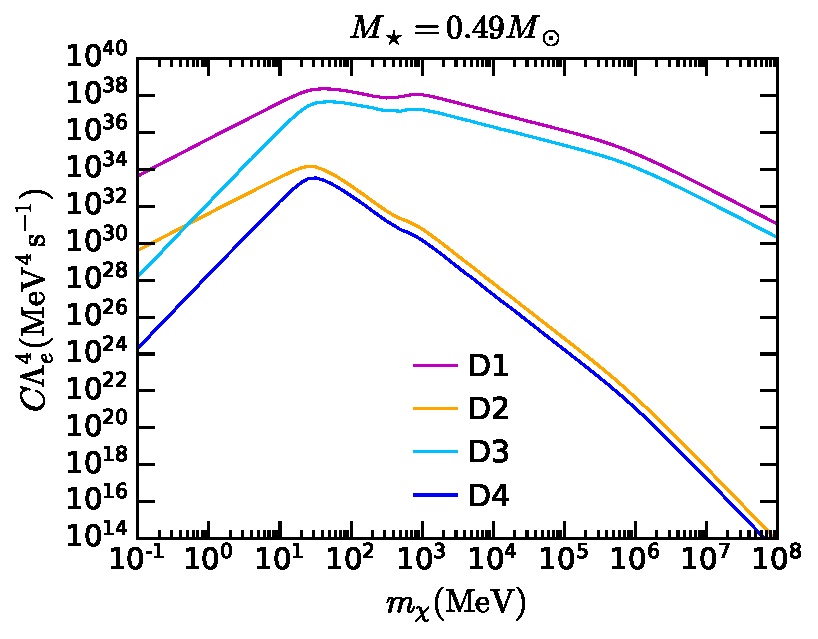
\includegraphics[width=0.49\textwidth]{wd_capture/C_mdm_optthin_e_0.49Msun_D1-D4.pdf}
    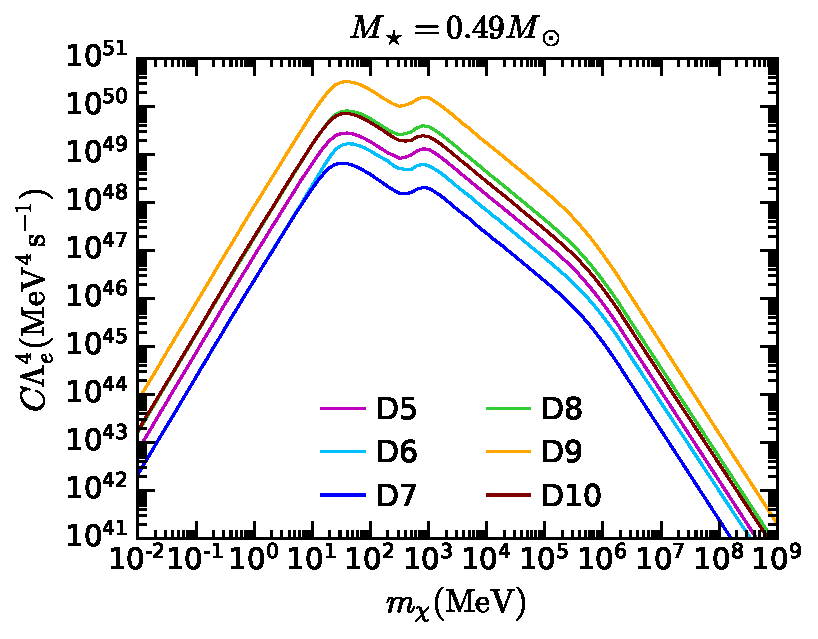
\includegraphics[width=0.49\textwidth]{wd_capture/C_mdm_optthin_e_0.49Msun_D5-D10.pdf} \\    
    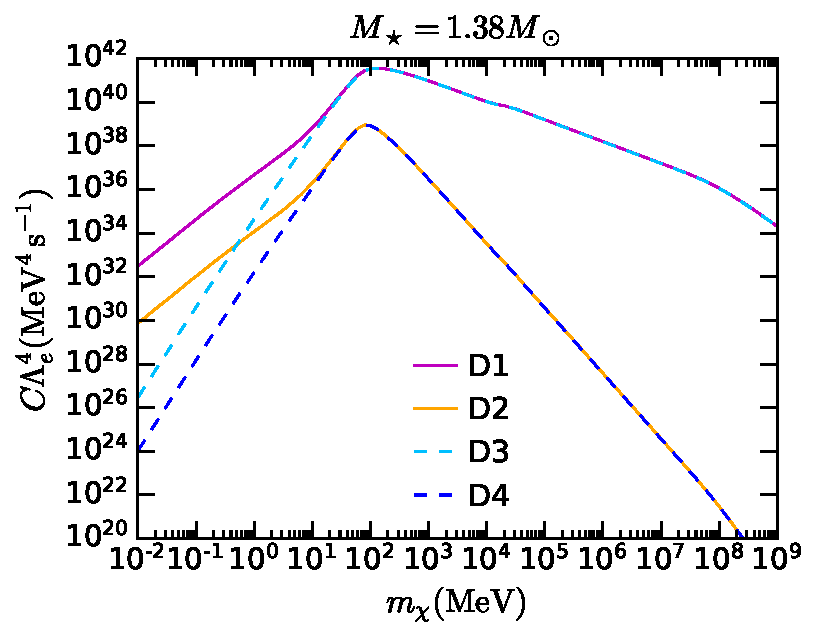
\includegraphics[width=0.49\textwidth]{wd_capture/C_mdm_optthin_e_1.38Msun_D1-D4.pdf}
    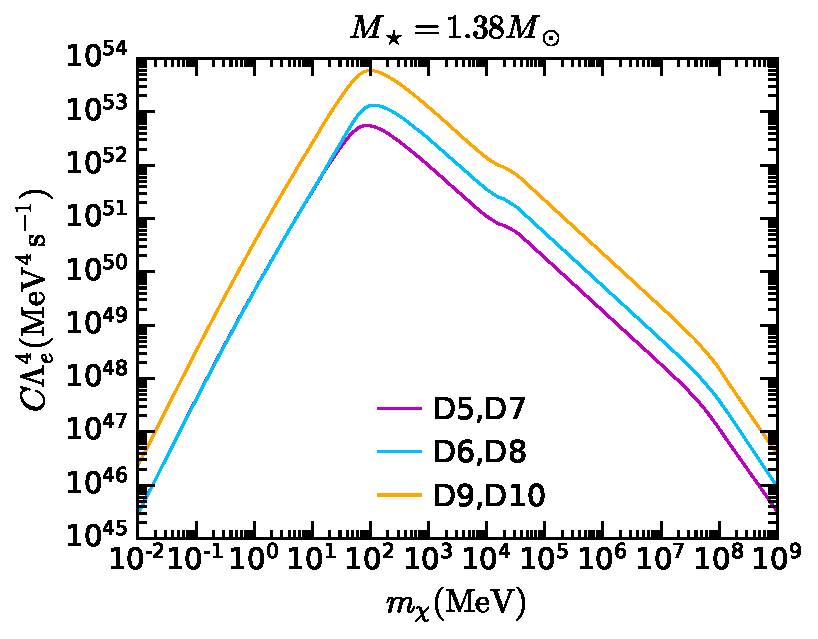
\includegraphics[width=0.49\textwidth]{wd_capture/C_mdm_optthin_e_1.38Msun_D5-D10.pdf} \caption{
 Capture rate for scattering on electrons, in the optically thin limit, as a function of the DM mass for  the lightest (WD$_1$, top panels) and heaviest (WD$_4$, bottom panels)  
 carbon WDs in Table~\ref{ch2:tab:WDs}.}
    \label{ch4:fig:Coptthinelec}
\end{figure}

%%%%%%%%%%%%%%%%%%%%%%%%%%%%%%%%%%%%%%%%%%%%%%%%%%%%%%%%%%%%%%%%%%%%%%%%%%%%%%%%%%%%
\subsubsection{Capture Rates for Electron Scattering}
\label{ch4:subsubsec:resutls_capture_WD}
%%%%%%%%%%%%%%%%%%%%%%%%%%%%%%%%%%%%%%%%%%%%%%%%%%%%%%%%%%%%%%%%%%%%%%%%%%%%%%%%%%%%

We are now ready to calculate the capture rate for the operators in Table~\ref{ch1:tab:opers_defn_full}, for DM-electron interactions with $\Lambda_f=\Lambda_e$, $\mu=m_\chi/m_e$ and the coefficients $c_N^I$, $I=S, P,V,A,T$ set to 1.
In Fig.~\ref{ch4:fig:Coptthinelec}, we present our results for $C\Lambda_e^4$ in the zero temperature and optically thin limits for carbon WDs with $\Mstar=0.49\Msun$ (top panels) and  $\Mstar=1.38\Msun$ (bottom panels). In both WDs, Pauli blocking strongly suppresses the capture rate in the light mass regime,  $m_\chi\lesssim 100\MeV$. Above this mass range, Pauli suppression persists but remains minimal.  

The change of slope in the Pauli suppressed region for operators D1 and D2 is due to their matrix elements containing a factor $(t-4m_e^2)$, which introduces an additional suppression due to the smallness of the electron mass in the $m_e\lesssim m_\chi\lesssim100\MeV$ interval~\cite{Bell:2020lmm_mar_ImprovedTreatmentDark}. This was also present in the NS case discussed in the previous section. 
Then, a transition between the Pauli blocked and the unsuppressed capture rate is observed for all the operators, which is immediately noticeable in the case of the light WD, where we observe a valley  in the  $100\MeV\lesssim m_\chi\lesssim1\GeV$ mass range. In the heavy WD, this transition region extends up to $\sim10\GeV$ and is more evident for operators D5-D10. 
The region at which multiple scattering becomes relevant also depends on the star configuration.  It occurs at $m_\chi\gtrsim1\TeV$ for the light WD, and at around  $m_\chi\gtrsim10^5\GeV$ for the heavy WD, observed as a change of slope in the capture rate at around those masses. 

It is worth remarking that, compared to the light WD, the heavy WD features an electron chemical potential more than one order magnitude higher, and that the electrons here are ultra-relativistic. As a result, the capture rate curves for WD$_4$ exhibit similar features to those observed in neutron stars where electrons are degenerate and ultra-relativistic~\cite{Bell:2020lmm_mar_ImprovedTreatmentDark}. In addition, since the electrons in the heavy WD are relativistic, the scattering amplitudes are dominated by terms of the form $t^ns^m$  in the large DM mass regime, while terms proportional to $m_e^2$ are suppressed (see Table~\ref{ch1:tab:opers_defn_full}). This results in very similar capture rates for operators D1 and D3. Likewise for the pairs (D2 and D4), (D5 and D7), (D6 and D8), and (D9 and D10).  

Finally, we note that the capture rate due to scattering on electrons would scarcely be affected by a different chemical composition, such as He or O.




%%%%%%%%%%%%%%%%%%%%%%%%%%%%%%%%%%%%%%%%%%%%%%%%%%%%%%%%%%%%%%%%%%%%%%%%%%%%%%%%%%%%
\subsection{Finite Temperature Effects and Evaporation}
\label{ch4:subsec:evapelectrons}
%%%%%%%%%%%%%%%%%%%%%%%%%%%%%%%%%%%%%%%%%%%%%%%%%%%%%%%%%%%%%%%%%%%%%%%%%%%%%%%%%%%%

% Compared the the NSs considered in the previous section, the core temperatures of WDs can be orders of magnitude higher, ranging between $\sim 10^5-10^8\K$. It is then reasonable to ask how important finite temperature effects are on the capture rate. 
% To determine the core temperatures of observed WDs, we need to know the atmospheric composition, especially the hydrogen content.  This is done using spectroscopic observations, (which are not available for WDs in M4), and model atmospheres. For the faintest (hence the oldest) and heaviest WDs in M4, a temperature of $\Tstar=10^5\K$ is consistent with the age estimated for the globular cluster, using the evolutionary sequences given in Ref.~\cite{Bedard_oct_Spectralevolutionhot}\footnote{See Section~\ref{ch2:subsec:WD_obs} for more details.}.


As was observed in the case of DM scattering off electrons in NSs, accounting for the finite temperature of the star can have a large impact when the dark matter mass is low. There are two main effects to consider. First, there is a boost in the capture and interaction rates as there is a greater volume of phase space for the interactions to take place in. 
This is due to the DM energy loss, $q_0$, being bounded from above such that $\qomax\lesssim3\MeV$ at zero temperature, and so only the outer shell of the Fermi sphere contributes to the capture rate. 
In comparison, non-zero $T_\star$ allows deeper shells of the Fermi sphere to contribute, substantially iincreasing the capture rate. 
Calculating the capture rate for finite $\Tstar$ is achieved by using the full form of the  Fermi-Dirac distributions in Eq.~\ref{ch4:eq:omegampauliur}, instead of approximating them with $\Theta$-functions, and removing the upper limit on the $E_e$ integration interval. 


Second, evaporation of the captured DM becomes possible due to scattering off the thermal electrons. Note that this is a purely thermal effect as in the zero-temperature approximation, the electron has no energy to impart to the DM, and hence, upscattering cannot occur.  Again, this is relevant for low-mass DM. 
For these finite temperature effects to be relevant in DM capture, they need to come into effect at DM masses above the evaporation mass of the WD~\cite{Garani:2018kkd_may_NewAnalysisNeutron, Bell:2020lmm_mar_ImprovedTreatmentDark}. 
To estimate the evaporation rate, we use  the full expression  obtained in Section~\ref{ch4:subsec:finite_temp_NS} for neutron stars, reiterated here for electrons in WDs
\begin{equation}
E \sim  \frac{ m_\chi m_e^2\sigma_{e\chi}}{4\pi^2} \left(\frac{1}{\sqrt{B(0)}}-1\right)^2  \exp\left[{-\frac{m_\chi}{\Tstar}}\left(\frac{1}{\sqrt{B(0)}}-1\right)\right],  
\label{ch4:eq:evap_WD}
\end{equation}
when the accreted DM is confined close to the centre of the star. 
Note that the evaporation rate is driven by the ratio $m_\chi/\Tstar$, and as such is enhanced for light DM. 

\begin{figure}[t!bp]
    \centering
  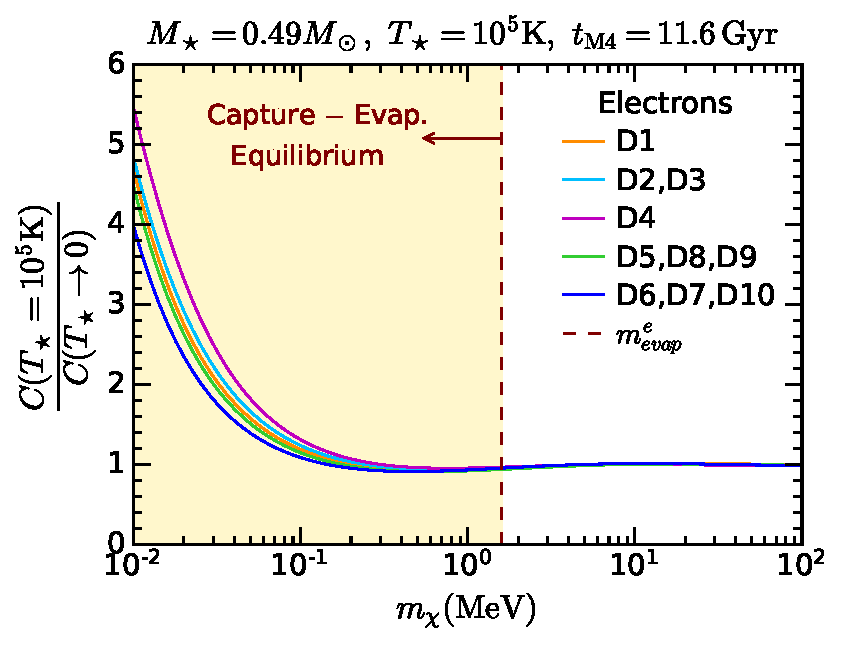
\includegraphics[width=0.495\textwidth]{wd_capture/R_CT_mdm_10_5K_D1_D10_e_M4S_0.49Msun.pdf}
  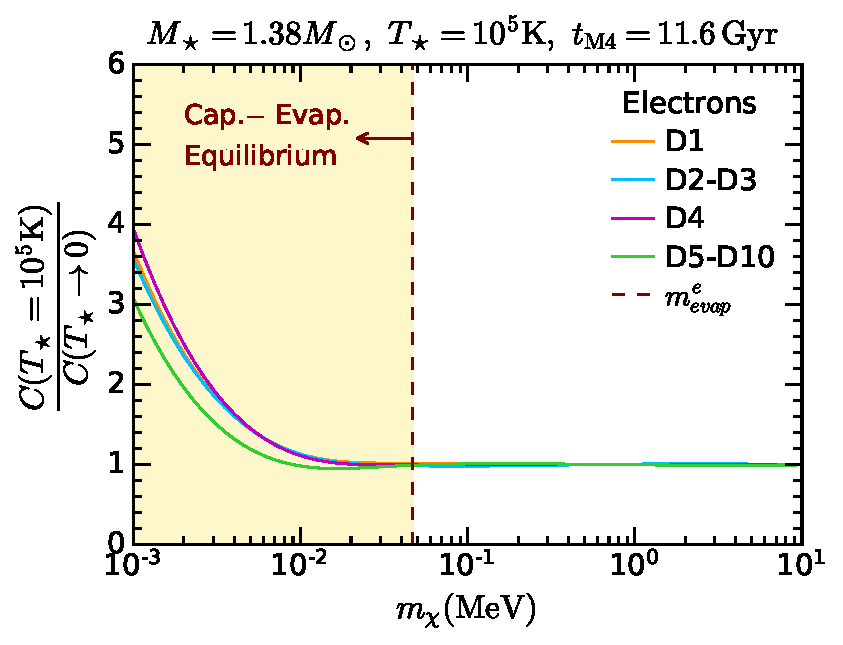
\includegraphics[width=0.495\textwidth]{wd_capture/R_CT_mdm_10_5K_D1_D10_e_M4S_1.38Msun.pdf} 
    \caption[Finite temperature effects on the capture rate in the case of scattering on electron targets, for two WDs in the globular cluster M4, namely WD$_1$ (left) and WD$_4$ (right) in Table~\ref{ch2:tab:WDs}.]{Finite temperature effects on the capture rate in the case of scattering on electron targets, for two WDs in the globular cluster M4, namely WD$_1$ (left) and WD$_4$ (right) in Table~\ref{ch2:tab:WDs}. The DM mass range where capture and evaporation are expected to be in equilibrium is shaded in yellow. The dashed brown line corresponds to the evaporation mass.}
    \label{ch4:fig:capTfinelec}
\end{figure}


In Fig.~\ref{ch4:fig:capTfinelec}, we plot the ratio of the capture rate for $\Tstar=10^5\K$ to the zero temperature approximation for the same WDs as in Fig.~\ref{ch4:fig:Coptthinelec}. Operators that depend only on powers of the exchanged momentum $t$, namely D1-D4, are the most affected by finite temperature corrections, followed by operators that contain in their matrix elements linear terms of the form $t^n s^m$, i.e., D5-D10. As can be noticed, the DM mass range at which these effects become relevant depends on the specific WD configuration and similar to the NS case is always below the evaporation mass for electron scattering $m_\mathrm{evap}^e$ (dashed brown lines).  We find that the evaporation mass for carbon WDs with  $\Tstar=10^5\K$ ranges from $m_\mathrm{evap}^e\sim 50\keV$ ($\Mstar=1.38\Msun$, right panel) to $m_\mathrm{evap}^e\sim 1.5\MeV$ ($\Mstar=0.49\Msun$, left panel). 
The evaporation mass is larger in warmer WDs, e.g. $\Tstar=10^6\K$, with an increase of one order of magnitude in $\Tstar$ resulting in a similar rise in $m_\mathrm{evap}^e$.  

%%%%%%%%%%%%%%%%%%%%%%%%%%%%%%%%%%%%%%%%%%%
%%%%%%%%%%%%%%%%%%%%%%%%%%%%%%%%%%%%%%%%%%%
\subsection{DM Induced Heating of WDs in GC M4}
\label{ch4:subsec:WD_results}
%%%%%%%%%%%%%%%%%%%%%%%%%%%%%%%%%%%%%%%%%%%
%%%%%%%%%%%%%%%%%%%%%%%%%%%%%%%%%%%%%%%%%%%




In this section, we calculate bounds on the cutoff scale of the dimension 6 EFT operators that describe DM interactions with electrons in WDs. To that end, we use the observed luminosity of the faintest WDs in the globular cluster M4~\cite{Bedin:2009it_jun_Endwhitedwarf,McCullough:2010ai_CaptureInelasticDark}, together with the estimations for $\rho_\chi$, $\vstar$ and $v_d$ derived in Ref.~\cite{McCullough:2010ai_CaptureInelasticDark}.  We compute the capture rate in the optically thin limit, assuming that the WDs are made of $\ce{^{12}C}$. Even though colder WDs have been recently observed by the Gaia mission~\cite{GentileFusillo_feb_GaiaDataRelease}, no significant bounds can be derived from this data due to the low DM density in the solar neighbourhood. 


Once captured, the gravitationally bound DM will continue to scatter with the WD constituents until they reach thermal equilibrium. We have checked the thermalisation timescales for scattering on electrons using the method described in Ref.~\cite{Bertoni:2013bsa_dec_DarkMatterThermalization}. We find that the longest time required for the DM to thermalize is $\sim 10^{5}$ yrs for any of the operators of interest.

Following thermalisation, the DM can self-annihilate in the WD interior. As in the for capture in the Sun discussed in Section~\ref{ch1:sec:solar_signals}, the number of DM particles present in the WD core evolves as
\begin{equation}
    \frac{dN_\chi}{dt} = C - A N_\chi^2, 
    \label{ch4:eq:ndm}
\end{equation}
where the coefficient $A$ is related to the annihilation rate through
\begin{equation}
 \Gamma_\mathrm{ann} =  \frac{1}{2}A N_\chi^2,   
\end{equation}
and we have assumed that evaporation is negligible, i.e., $m_\chi\geq m_{evap}$. 
The annihilation coefficients can be calculated from the thermally averaged annihilation cross-sections for each operator that can be found in Ref.~\cite{Zheng:2010js_Constraininginteractionstrength}.

To calculate these cross-sections, we only consider DM annihilating to SM leptons at tree level, as there is no a priori reason to expect similar-scale DM couplings to quarks. In principle, one would have two cutoff scales for DM coupling to the quark and lepton sectors, with the relationship between the two depending on the UV physics. 
This means that when computing bounds on $\Lambda_e$ for interactions with electrons, no assumptions were made regarding the strength of DM-quark interactions. 
Instead, loop-induced effective couplings to quarks were calculated similarly to Refs.~\cite{Kopp:2009et_DAMALIBRAleptonically,Bell:2019pyc_jun_CaptureLeptophilicDark}.  
Importantly, note that below the electron mass annihilation to neutrinos or loop-induced annihilation to photons (non-zero only for some operators) are the only allowed annihilation channels. 

If the capture and annihilation processes are in equilibrium, then $\Gamma_{ann}=C/2$ and the DM contribution to the star luminosity is $L_\chi=m_\chi C(m_\chi,\Lambda_f)$. The time in which this equilibrium is reached is determined by the steady-state solution of Eq.~\ref{ch4:eq:ndm}, and is given by
\begin{equation}
    \tau_\mathrm{eq} = \frac{1}{\sqrt{C A}}.\label{ch4:eq:taueq}
\end{equation}
We can then set the EFT cutoff $\Lambda_e$ to the values obtained from the WD luminosity (see paragraph below)  to calculate the corresponding equilibrium times and hence verify that capture-annihilation equilibrium is met. 


\begin{figure}[t!bp]
    \centering
    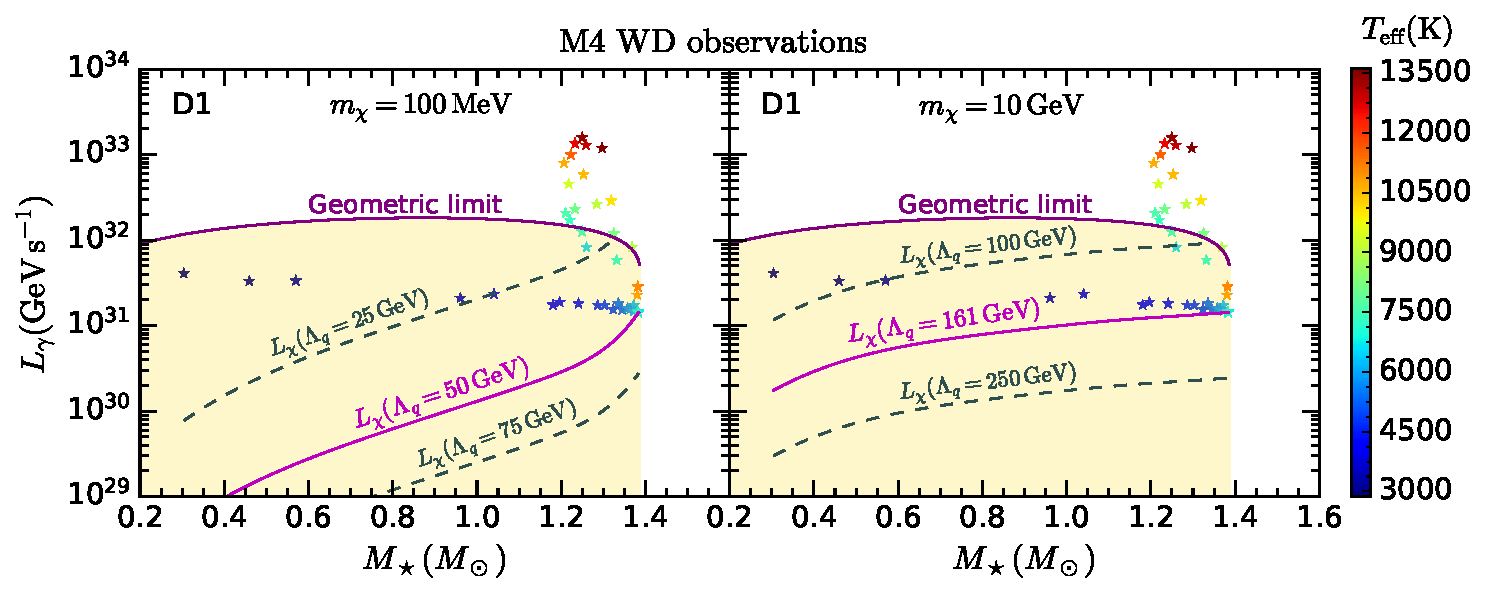
\includegraphics[width=\textwidth]{wd_capture/Lum_WDmass_M4.pdf}
    \caption[WDs observed in the globular cluster M4 and DM contribution to the star luminosity $L_\chi$ for different values of the cutoff scale $\Lambda_e$ and $m_\chi$ for D1.]{WDs observed in the globular cluster M4 and DM contribution to the star luminosity $L_\chi$ for different values of the cutoff scale $\Lambda_e$ and $m_\chi$ for D1. The red lines correspond to the maximum achievable $L_\chi$ for electron targets obtained in the geometric limit. The blue lines represent the minimum value of $\Lambda_e$ that is consistent with the WD observations. }
    \label{ch4:fig:limitset}
\end{figure}


To estimate the limits on the cutoff scale $\Lambda_e$ for DM interactions with electrons, we compare the luminosity due to DM  with the WD observed luminosities $L_\gamma$. In Fig.~\ref{ch4:fig:limitset}, we illustrate how we have performed this calculation.
The observed luminosity of the WDs in M4 is shown in the $L_\gamma-\Mstar$ plane\footnote{Actually, there are more WDs observed in the globular cluster M4 than those shown in Fig.~\ref{ch4:fig:limitset}. We have given preference to the faintest WDs since these give the strongest constraints on the DM-electron cross-section.}, where we have used the luminosity and effective temperature to infer the radius of every star through the relation $L_\gamma = 4\pi \sigma_\mathrm{SB} \Rstar^2 T_\mathrm{eff}^4$ with $\sigma_\mathrm{SB}$ the Stefan-Boltzmann constant. 

Since there are no independent measures of the mass of the WDs in M4, and we require radial profiles of the target number density, electron Fermi energy, and escape velocity to compute capture and evaporation rates, we have solved the TOV equations coupled with the FMT EoS for carbon WDs to calculate $\Mstar$, as discussed in detail in Section~\ref{ch2:sec:FMT_EoS}.\footnote{The mass and radius obtained using this method are in good agreement with recent observations within 2~kpc retrieved from the Montreal White Dwarf Database~\cite{Dufour_mar_Montrealwhitedwarf}, which contains more than 32000 WDs identified by Gaia DR2~\cite{Torres_feb_GaiaDR2halo} and EDR3~\cite{Gaia:2020wqu_may_Gaiaearlydata}, and spectroscopy measurements from surveys including SDSS DR12 and 2MASS. See Fig.~\ref{ch2:fig:WD_mass_radius} for the comparison.}  We also show the DM luminosity for different values of $\Lambda_q$ for $m_\chi=100\MeV$ (left) and $m_\chi=10\GeV$ (right), calculated using different WD configurations. 

As seen in Fig.~\ref{ch4:fig:limitset}, the WD with $M_\star\simeq1.38 \Msun$ is the star that imposes a lowest bound on $\Lambda_q$ (solid blue line), since $L_\gamma$ should be at least equal to the expected contribution from DM for all the observed WDs. 
In other words, if the luminosity due to DM capture and annihilation is at most equal to the observed luminosity of the faintest and heaviest WD in M4 ($M_\star\simeq1.38 \Msun$), there will be no tension between these observations and DM-induced heating of the WDs. 
While the results in Fig.~\ref{ch4:fig:limitset} assume WDs of a pure carbon composition, we have checked that a pure He composition for stars of $\Mstar\lesssim0.5\Msun$ does significantly not alter the bounds on $\Lambda_e$. 
Note that the lower bounds are always well below the DM luminosity for maximal capture (geometric limit, see red lines). 
Lower values of $\Lambda_e$ (dashed grey lines) would be in tension with the lowest luminosity WDs. 



\begin{figure}[t!bp]
    \centering
    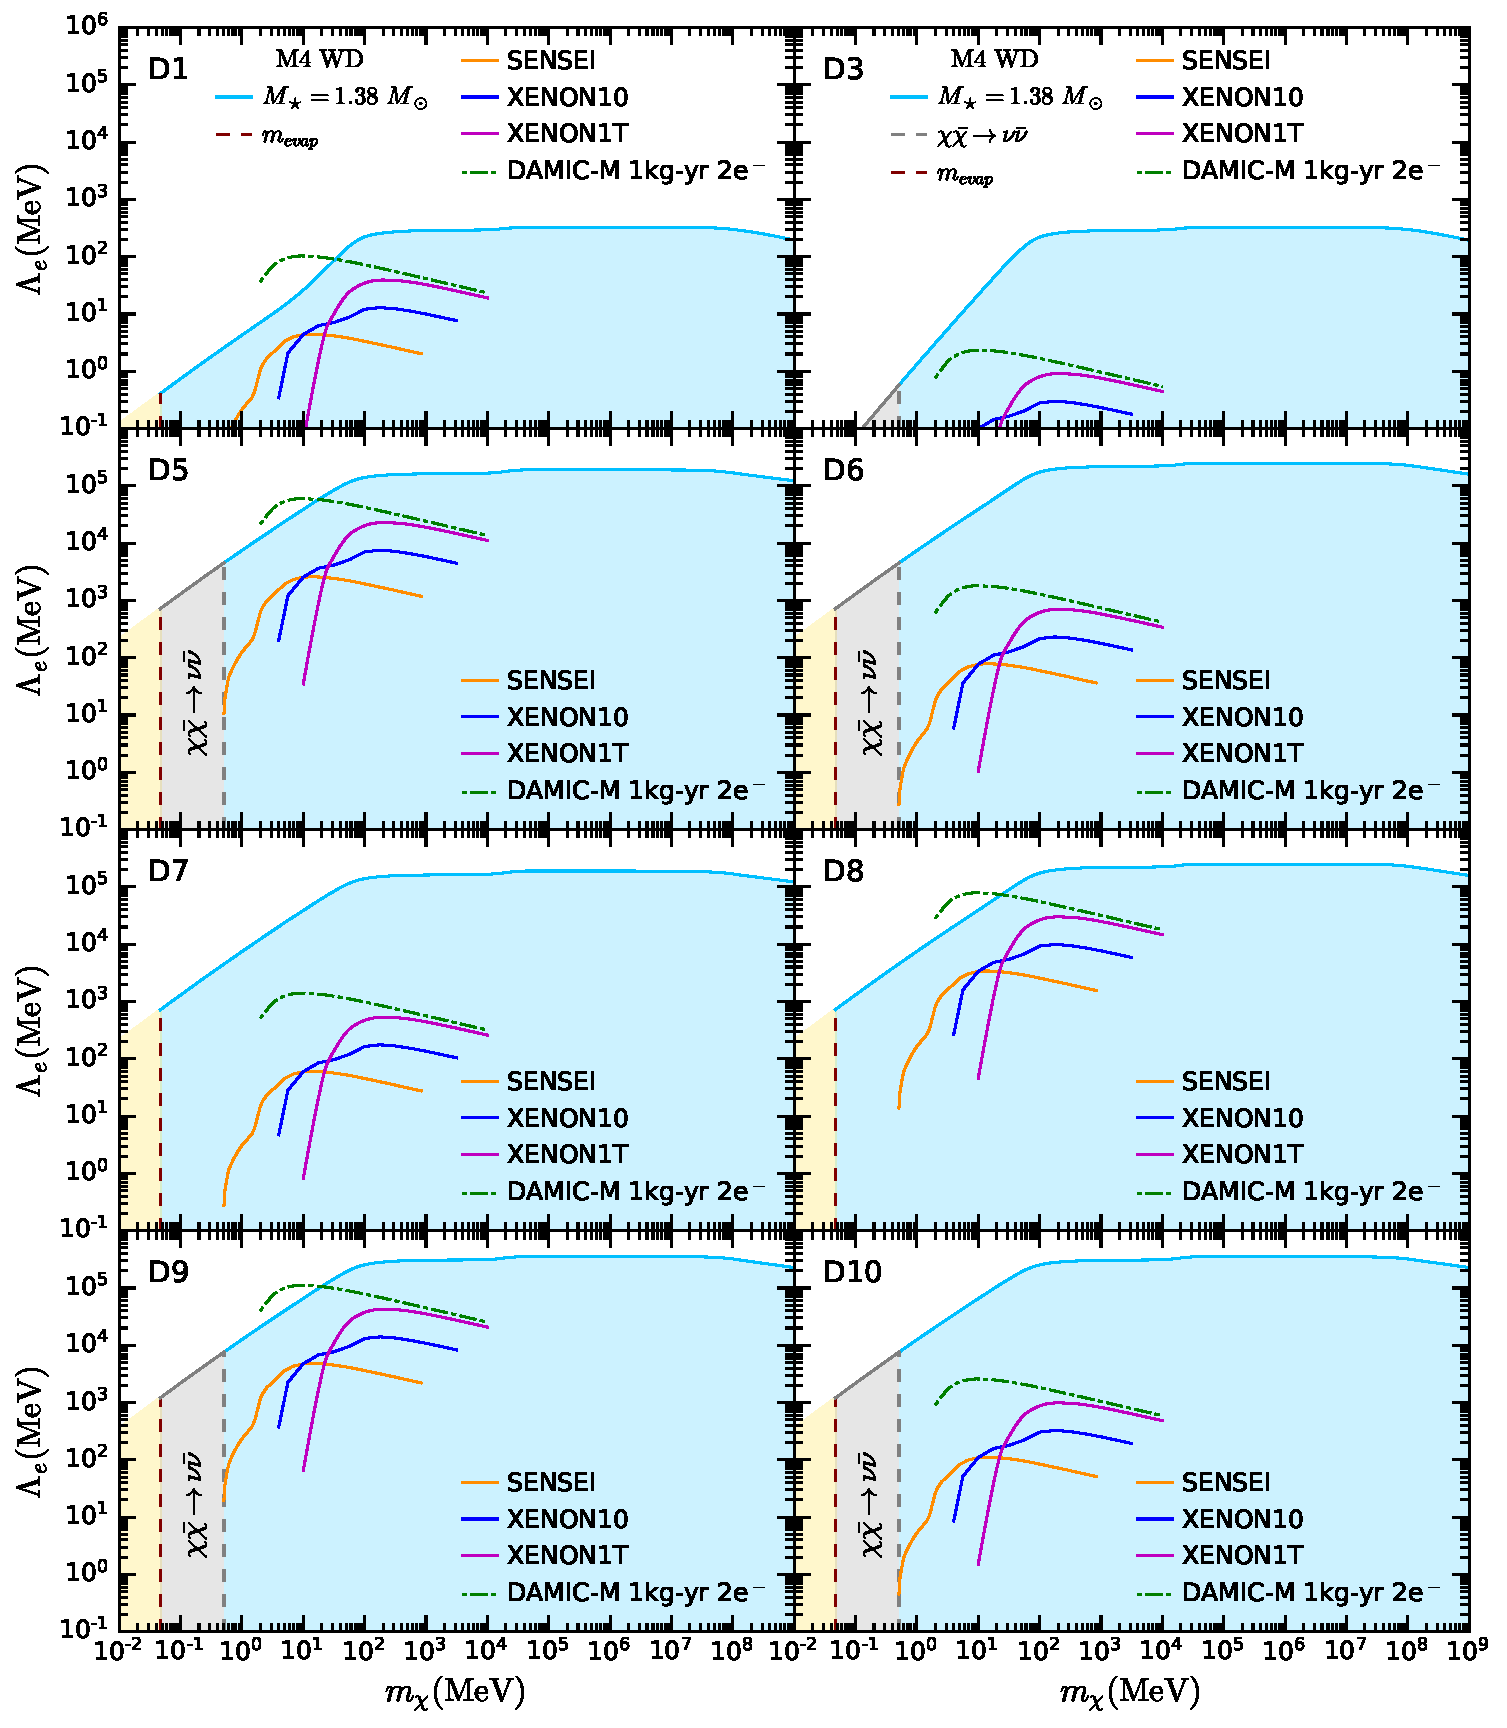
\includegraphics[width=0.8\textwidth]{wd_capture/Lambda_mdm_e_limits.pdf}
    \caption[Limits on $\Lambda_e$ for DM interactions with electrons for the WD with the lowest luminosity and heaviest WD in the globular cluster M4, assuming $\rho_\chi=798\GeV\cm^{-3}$ (contracted halo) \cite{McCullough:2010ai_CaptureInelasticDark} and $\Tstar=10^5\K$.]{Limits on $\Lambda_e$ for DM interactions with electrons for the same WD obtained with the lowest luminosity and heaviest WD in the globular cluster M4, assuming $\rho_\chi=798\GeV\cm^{-3}$ (contracted halo) \cite{McCullough:2010ai_CaptureInelasticDark} and $\Tstar=10^5\K$. The region where capture and evaporation (for $\Tstar=10^5\K$) are expected to be in equilibrium is shaded in yellow, and the region where DM annihilates to neutrinos that escape the WD is shaded in grey. For comparison, we show upper bounds from the leading electron recoil experiments for heavy mediators from SENSEI~\cite{SENSEI:2020dpa_SENSEIDirectdetectionresults}/DAMIC~\cite{DAMIC:2019dcn_Constraintslightdark}, Xenon10~\cite{Essig:2017kqs_Newconstraintsprospects}, Xenon1T~\cite{XENON:2019gfn_Lightdarkmatter} and the projected sensitivity for DAMIC-M~\cite{Essig:2015cda_DirectdetectionsubGeV}. }
    \label{ch4:fig:Llimitse}
\end{figure}


In Fig.~\ref{ch4:fig:Llimitse}, we show the limits on the cutoff scale $\Lambda_e$, in the case where DM is captured solely by collisions with the degenerate electrons. The shaded blue regions are the excluded parameters.
For operators D1-D4, for which the squared matrix elements
depend exclusively on the transferred momentum $t$, the DM-electron couplings is proportional to the tiny electron Yukawa coupling. 
This reduces the capture rate in such a way that for operator D4, the bounds on $\Lambda_e$ lie entirely in the $\Lambda_e \lesssim m_\chi$ region, and for D2 only a small corner of the allowed parameter space surpasses this threshold. Given these low limits on the EFT cutoff scale $\Lambda_e$, such that an EFT description would not be valid, we do not plot results for D4 or D2.

For the remaining operators, especially D5-D10, there is a much larger region of parameter space where the limits on $\Lambda_e$ are such that an EFT description would be valid. In all cases, the lower limits on $\Lambda_e$, obtained using the WD with $\Mstar=1.38\Msun$ in M4, surpass the leading bounds from electron recoil experiments by at least $\sim$ an order of magnitude.  In most cases, they even surpass the projected sensitivity for the future experiment DAMIC-M (with the exceptions being D1, D5, D8 and D9 in the region below $m_\chi\lesssim10\MeV$ -- see dot-dashed green lines). DM scattering on electrons
is heavily hampered by Pauli blocking for  $m_\chi\lesssim100\MeV$.  

The reach in the light DM mass regime is restricted by the evaporation mass for operators D1, D7, and D8 (see yellow region) and the electron mass for D3, D5, D6, D9 and D10 (see region shaded in grey) where DM annihilation to neutrinos is either the only final state allowed or the dominant channel.  Despite those limitations, we conclude that constraints from the observed luminosity of cold faint WDs in old globular clusters that have been able to retain their initial DM content in the innermost region of the cluster, can potentially exclude larger regions of the parameter space than direct detection, particularly in the sub-GeV region. This is especially relevant for leptophilic DM models.

\begin{figure}
    \centering
  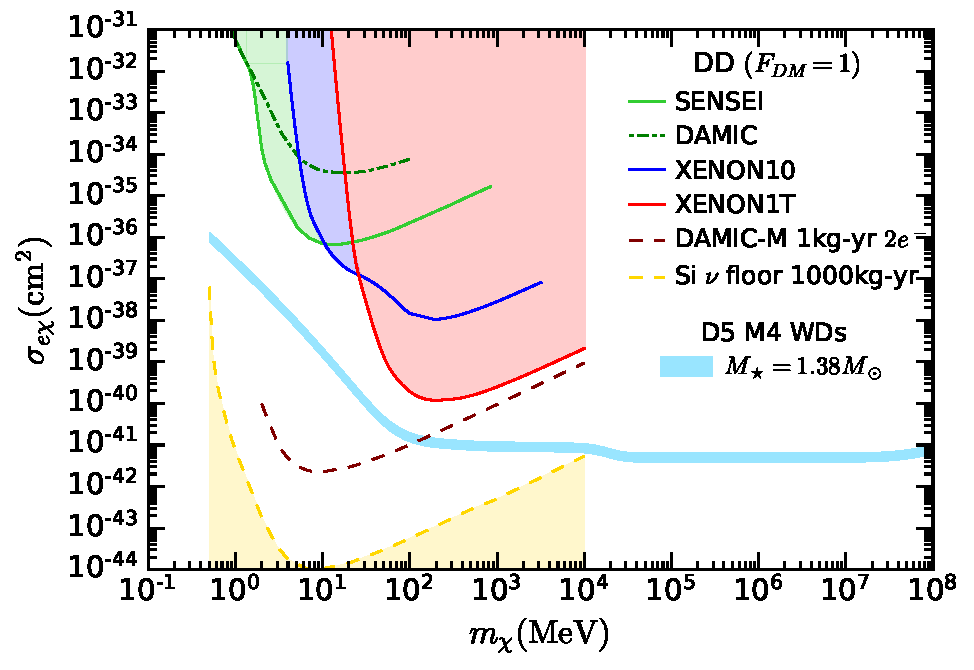
\includegraphics[width=0.7\textwidth]{wd_capture/DD_WD_electrons_D5.pdf}
    \caption[Upper bounds on the DM-electron scattering cross-section for D5.]{Upper bounds on the DM-electron scattering cross-section for D5. The light blue band represents the limit from the WD observations in M4. The width fo this band denotes the uncertainty in the DM density in M4~\cite{McCullough:2010ai_CaptureInelasticDark}.  
     For comparison, we show leading electron recoil bounds for heavy mediators from SENSEI~\cite{SENSEI:2020dpa_SENSEIDirectdetectionresults}, DAMIC~\cite{DAMIC:2019dcn_Constraintslightdark}, Xenon10~\cite{Essig:2017kqs_Newconstraintsprospects}, Xenon1T~\cite{XENON:2019gfn_Lightdarkmatter}, the projected sensitivity for DAMIC-M~\cite{Essig:2015cda_DirectdetectionsubGeV}, and the neutrino floor for silicon detectors~\cite{Essig:2018tss_Solarneutrinossignal}. 
    }
    \label{ch4:fig:D5sigmalimit}
\end{figure}


Finally, in Fig.~\ref{ch4:fig:D5sigmalimit}, we conservatively compare the bound on the scattering cross-section of the vector-vector operator D5 obtained from WDs in M4, with the limits from electron recoil experiments. Even though the WD constraint is not able to probe the region where neutrino coherent scattering is expected to hamper the sensitivity of silicon detectors or extend down below the electron mass, it would certainly surpass current DD bounds by orders of magnitude in $\sigma_{e\chi}$. It would even surpass the projected sensitivity for DAMIC-M, especially in the sub-MeV regime where no projections have been made\footnote{In the sub-MeV DM mass regime, modest limits on the DM-electron scattering cross-section can be obtained by considering DM upscattered by cosmic rays. See, e.g. Refs.~\cite{Cappiello:2018hsu_Reversedirectdetection,Ema:2018bih_Lightdarkmatter,Dent:2020syp_oct_Presentfuturestatus}.}, despite the reduced WD sensitivity in this region due to Pauli blocking. 

%%%%%%%%%%%%%%%%%%%%%%%%%%%%%%%%%%%
%%%%%%%%%%%%%%%%%%%%%%%%%%%%%%%%%%%
\section{Summary}
\label{ch4:sec:summary}
%%%%%%%%%%%%%%%%%%%%%%%%%%%%%%%%%%%
%%%%%%%%%%%%%%%%%%%%%%%%%%%%%%%%%%%

In this chapter, we have applied the formalism for dark matter capture in compact objects discussed in Chapter~\ref{chapter:capture_intro} to leptonic targets. Namely, we looked at DM scattering from electrons an muon in NSs, as well as electrons in WDs.

In the NS case, we saw that capture from muon targets was qualitatively similar to the neutron target case of Section~\ref{ch3:sec:results}. On the other hand, capture from electrons for a subset of the EFT operators exhibits interesting behaviour in the low DM mass regime due to their ultrarelativistic nature. We then projected the sensitivity to the DM-lepton scattering cross-section, $\sigmathl$, that a future observation of an old, cold NS might be able to achieve. When these results are compared to current and upcoming direct detection experiments, we find that NSs have the potential to probe regions of this parameter space orders of magnitude below current constraints. 

In terms of the electrons in WDs, we took advantage of the existing catalogue of WD observations in globular cluster M4 to explore the impact of DM heating in these stars. We find that requiring that the luminosity induced by the kinetic and annihilation heating from the captured DM not exceed the observed luminosities of the WDs, we can constrain the DM-electron scattering cross-section over a wide DM mass range. In fact, despite the considerable suppression from Pauli blocking, limits from DM heating are shown to surpass direct detection constraints and probe deep into the neutrino floor. 
We note that these limits are dependent on M4 containing dark matter, which in turn depends on M4 having been formed within a DM sub-halo. The exact mechanism by which M4 was formed is still unknown and may have instead formed due to an intermediate-mass black hole, forgoing the need for the DM sub=halo ~\cite{Vitral}. If this were the case, and the DM density of M4 was similar to our local density of $0.4 \GeV \cm^{-3}$, then we would not be able to observe the effects of DM heating on the WDs. Hence, no limits could be placed. 

We now move on from scattering off point-like objects to consider capture from baryons in NSs. Here, we will need to account for both their finite size and correctly treat them as a strongly interacting medium. 